\chapter{Results}

\section{Code validation}
It is of great importance to us that the implementation is free of any errors that might yield wrong results.
In order to guarantee this we perform a number of tests, of which results are known prior to running the calculations.

\subsection{Hand calculation}
First we consider non-interacting particles, where the total energy is simply the sum of single-particle energies, as seen in eq.~\eqref{eq:manybody:nonInter}.
The first filled shell have two electrons with $\hbar \omega$ as the energy, the next four electrons with an energy of $2\hbar \omega$ each, and so on.
A shell has two more electrons than the previous, each electron with an energy of $\hbar \omega$ more than an electron on the previous shell.
The total uncorrelated energy of $F$ filled shell is thus
\begin{equation}
E_{Uncorr} = 
2 \cdot 1\hbar \omega 
+ 
4 \cdot 2\hbar \omega 
+
\cdots
+
2F \cdot F\hbar \omega
=
\sum_{i=1}^F 2 i^2 \hbar\omega , 
\end{equation}
a series that can be recognized as 
\begin{equation}
E_{Uncorr} = \frac{2F^3 + 3F^2 + F}{3} \hbar \omega .
\end{equation}
Energies for the first 7 filled shells for different values of $\omega$ is found in table~\ref{tab:results:Euncorr}.
\begin{table}
\begin{center}
\caption{Uncorrelated energies for the first seven filled shells for different values of $\omega$. Energies are measured in Hartrees.}
\label{tab:results:Euncorr}
\begin{tabular}{l|rrrrrrr}
\hline
E     &    1  &   2  &   3    &  4   &  5    &  6    &  7   \\
\hline \hline
1.0   &   2.0 & 10.0 & 28.0   & 60.0 & 110.0 & 182.0 & 280.0 \\
0.9   &   1.8 &  9.0 & 25.2   & 54.0 &  99.0 & 163.8 & 252.0 \\
0.8   &   1.6 &  8.0 & 22.4   & 48.0 &  88.0 & 145.6 & 224.0 \\
0.7   &   1.4 &  7.0 & 19.6   & 42.0 &  77.0 & 127.4 & 196.0 \\
0.6   &   1.2 &  6.0 & 16.8   & 36.0 &  66.0 & 109.2 & 168.0 \\ 
0.5   &   1.0 &  5.0 & 14.0   & 30.0 &  55.0 &  91.0 & 140.0 \\
0.4   &   0.8 &  4.0 & 11.2   & 24.0 &  44.0 &  72.8 & 112.0  \\
0.3   &   0.6 &  3.0 &  8.4   & 18.0 &  33.0 &  54.6 &  84.0  \\
0.2   &   0.4 &  2.0 &  5.6   & 12.0 &  22.0 &  36.4 &  56.0 \\
0.1   &   0.2 &  1.0 &  2.8   &  6.0 &  11.0 &  18.2 &  28.0  \\
\hline \hline
\end{tabular}
\end{center}
\end{table}
These energies must be reproduced by both the Hartree-Fock (HF) and coupled-cluster programs. 
In order to test this we simply use an empty two-particle element file when running our program, thus leaving all matrix elements at their initialized value, zero.


\paragraph{}
For two particles it is possible to do calculations by hand if restricted to a small basis.
The simplest is to use a total of six basis functions, the first two shells, where the first shell is filled by the two particles.
Coupled cluster should, including single and double excitations, be able to account for all possible determinants in this case, and therefore yield same result as eigenvalues obtained by diagonalization of the full Hamilton matrix.
The determinants will now have $n=0$, allowing us to write determinants as $|m^pm_s^p;m^qm_s^q\rangle$ the reference determinant is either 
\begin{equation}
|0\downarrow;0\uparrow\rangle ,\textrm{ or } |0\uparrow;0\downarrow\rangle .
\end{equation}
Only excitations preserving $M=0$ and $M_s=0$ from the ground state are allowed, restricting possible determinants to, 
\begin{equation}
\begin{matrix}
|0\downarrow;0\uparrow\rangle ,  &  |0\uparrow;0\downarrow\rangle , \\
|-1\downarrow;+1\uparrow\rangle , & |+1\uparrow;-1\downarrow\rangle , \\
|+1\downarrow;-1\uparrow\rangle ,  &  |-1\uparrow;+1\downarrow\rangle . 
\end{matrix}
\end{equation}
The left column have the same states as in the right, except for the two particles being swapped, at most raising a negative phase factor, allowing us to skip half of the states.
Omitting the explicit spin notation, restricted to only the three left states, the Hamiltonian to solve is,
\begin{equation}
\hat{H}
=
\begin{bmatrix}
2\omega + \langle 0;0||0;0\rangle 
   &  \langle 0;0||-1;+1\rangle  
   & \langle 0;0||+1;-1\rangle \\
\langle-1;+1||0;0\rangle 
   & 4\omega + \langle-1;+1||-1;+1\rangle 
   &  \langle-1;+1||+1;-1\rangle    \\
\langle+1;-1||0;0\rangle 
   & \langle+1;-1||-1;+1\rangle 
   & 4\omega + \langle+1;-1||+1;-1\rangle    \\
\end{bmatrix} , 
\end{equation}
or 
\begin{equation}
\hat{H}
=
\begin{bmatrix}
3.2533 & 0.3133 & 0.3133 \\
0.3133 & 4.8617 & 0.2350 \\
0.3133 & 0.2350 & 4.8617 
\end{bmatrix},
\end{equation}
for $\omega=1$.
This matrix has the lowest eigenvalue
\begin{equation}
E_0 = 3.1523,
\end{equation}
a result that is perfectly reproduced by our implementation, even when including more decimals. 
It is possible to do hand calculations also for three shells, as in \cite{marte}, resulting in 
\begin{equation}
E_0 = 3.0386,
\end{equation}
also reproduced.



\subsection{Effective interaction}
For two electrons the exact result is known to be $E_0 = 3[Ha]$~\cite{mtaut}, a result we would like the two-particle case to converge towards.
A standard interaction is the integral of the Coulomb repulsion, unfortunately shown to converge slowly as a function of the size of basis. 
For this reason we investigate the use of an effective interaction, previously used with great success first in nuclear physics and later also for quantum dots~\cite{PhysRevB.84.115302}.

An effective interaction is obtained by solving the two-particle problem in an untruncated Hilbert space, and project the Hamiltonian into the truncated space by a similarity transform.
The lowest eigenvalue of this effective, truncated, Hamiltonian should now be the same as for the exact standard Hamiltonian in an infinite space.
For more than two particles we will no longer get the same eigenvalue, the idea, however, is that the contribution from two-particle interactions still are accounted more precisely than a standard interaction.
All two-particle elements, both for standard and effective interactions, are written to a file using the OpenFCI~\cite{openfci} library.

We test our program by running with one filled shell (two electrons) using an effective interaction, and observe how we get the exact values of $3[Ha]$ for $\omega=1$ and $1.658772[Ha]$ for $\omega= 0.5$, irrespective of the basis size.
In these tests we use an energy-cut model space shown in fig.~\ref{fig:results:energycut}, in principle suggesting that only half of the elements are used.
Despite yielding exact results for two particles this has shown convergence problems for larger systems~\cite{mplohne}, and we therefore use twice as big a basis when producing the interactions, and simply omit elements not suitable for the coupled-cluster approach.
At the cost of introducing an error, assumed to be fairly small in the case of a large basis, we gain better convergence.
\begin{figure}
\begin{center}
\caption{Energy-cut modelspace}
\label{fig:results:energycut}
\end{center}
\end{figure}



\subsection{Earlier results}
There is also a number of previously obtained results that we should be able to reproduce with our new program. We reproduce the results of Lohne~\cite{mplohne}, Hagen and Hjorth-Jensen~\cite{PhysRevB.84.115302} for HF and CCSD for both a Hartree-Fock and a harmonic-oscillator basis.

When it comes to Jørgensen's thesis~\cite{marte} we see inconsistencies, also discussed by the author, for calculations using a Hartree-Fock basis.
A thorough comparison of codes revealed how the single-particle part of the Hamiltonian, $\hat{h}^{0}$, was represented as a vector only storing the diagonal elements.
Being diagonal this works flawlessly in the case of a harmonic-oscillator basis, but will fail for a Hartree-Fock basis as we have no guarantee of a diagonal form after the transformation,
\begin{equation}
\hat{h}^{(0)} = C \hat{h}^{(0)} C^T , 
\end{equation}
as a state $|p\rangle$  may have mixed in other states from the same channel by the unitary transformation.

In all we either reproduce results or are able to explain why there are differences in the comparisons.



\section{Efficiency}
We like to believe that our implementation has pushed the boundary on what calculations are possible to run on a single node.
Multiple optimizations are done in order to get the program efficient without the penalty of loosing flexibility.
The main improvement is how all parts are now in terms of transition channels, reducing the dimensionality off all terms drastically.
Another improvement is seen by exploring different approaches to matrix multiplications. 

\subsection{Optimized matrix multiplication}
The main workhorse in this program is multiplication of matrices, whose dimension increases with increasing system size and basis.
In the coupled cluster machinery the most expensive term, eq.~\eqref{eq:CC:t2_t2_diag}, scales as $\dim(\xi)^2 \cdot \dim(\mu)$ for each block of a transition channel, multiplying two matrices of $\dim(\xi)\times\dim(\xi)$ and $\dim(\xi) \times \dim(\mu)$.
The widest channel, $M=M_s = 0$, has 2 hole-hole configurations for two particles, 6 hole-hole configurations for six particles (see fig.~\ref{fig:results:hhStatesF2}), and thereafter growing.
A more comprehensive list of the number of both hole-hole and particle-particle configurations in this channel is listed in table~\ref{tab:results:dimConfig0}
\begin{table}
\begin{center}
\caption{Listed are the number hole-hole configurations, $\max_{\lambda}\dim(\mu)$, and the number of particle-particle configurations, $\max_{\lambda}\dim(\xi)$, in the widest channel. The most expensive term for CCSD scales as $\left(\sim \max_{\lambda}\dim(\xi)^2 \max_{\lambda}\dim(\mu)\right)$, equal to $n_p^4 n_h^2$ if not using block diagonal matrices.}
\label{tab:results:dimConfig0}
\begin{tabular}{c|ccccccc}
 & 2 & 6 & 12 & 20 & 30 & 42 & 56 \\
\hline
20 & (2,2842) & (6,2766) & (16,2664) & (32,2528) & (58,2378) & (94,2198) & (144,2016)  \\
22 & (2,3764) & (6,3680) & (16,3566) & (32,3414) & (58,3244) & (94,3040) & (144,2830)  \\
24 & (2,4866) & (6,4774) & (16,4648) & (32,4480) & (58,4290) & (94,4062) & (144,3824)  \\
26 & (2,6164) & (6,6064) & (16,5926) & (32,5742) & (58,5532) & (94,5280) & (144,5014)  \\
28 & (2,7674) & (6,7566) & (16,7416) & (32,7216) & (58,6986) & (94,6710) & (144,6416)  \\
30 & (2,9412) & (6,9296) & (16,9134) & (32,8918) & (58,8668) & (94,8368) & (144,8046)  \\
\end{tabular}
\end{center}
\end{table}
\begin{figure}
\begin{center}
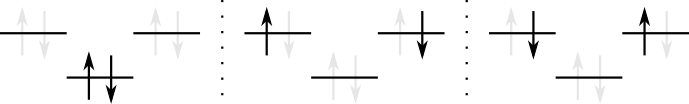
\includegraphics[scale=1.5]{../10-results/figs/hhStatesF2.png}
\caption{The three different hole-hole states with $M = M_s = 0$ for six particles. Counting the multiplicity of swapping the two particles there are six hole-hole states in total.}
\label{fig:results:hhStatesF2}
\end{center}
\end{figure}

\paragraph{}
We first test the different implementations of the `GEMM' class calculating the matrix product of two matrices, filled with random number, whose size corresponds to the widest channel of the most expensive term in the CC equations. 
In fig.~\ref{fig:results:timeMultCC} we see how the implementations perform for $2$, $12$, $30$ and $56$ electrons.
The `GEMM' base class is used with both Netlib and Goto's blas library as backend, Netlib running serially whereas Goto's implementation utilizes all four cores on the test machine, a stock Intel i7-920 clocked at 2.67 GHz.
Both Netlib and Goto blas have also been used with the `Strassen' sub class, conducting only one Strassen recursion, allowing us to identify whether such a recursion is beneficial or not.
AMD's APPML library is also used through the `CLgemm' class, which provides memory copying to and from device in addition to scheduling the blas routine.
To avoid running out of memory on the GPU we split the matrices by applying a Strassen recursion whenever matrices fills more than 90\% of the GPU.
This amount was chosen as a safety precaution, but could most likely be 100\%.
\begin{figure}
\begin{center}
\subfigure[$N=2$]{
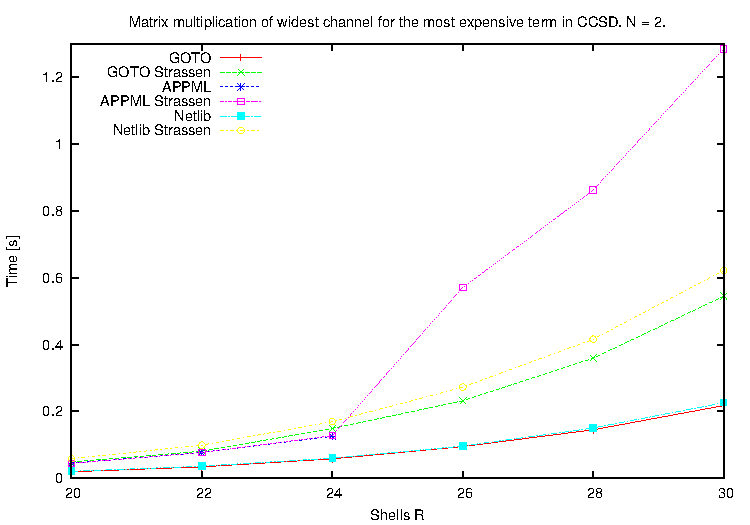
\includegraphics[scale=0.6]{../10-results/figs/timeMult/timeMultCC_1.pdf}
}
\subfigure[$N=12$]{
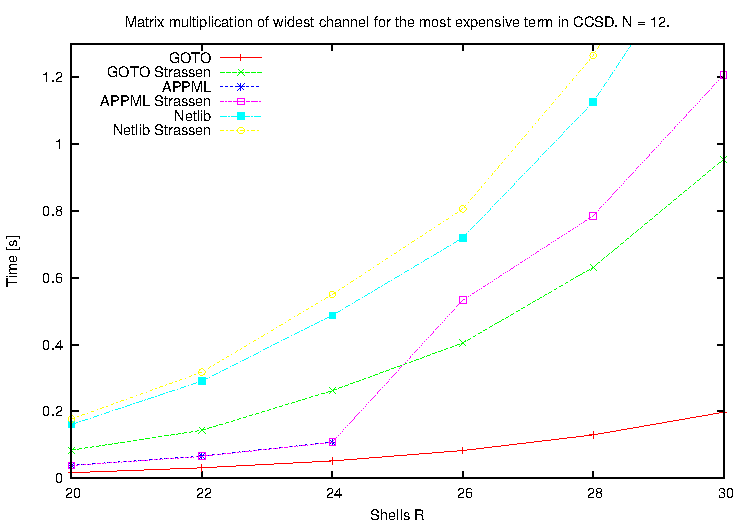
\includegraphics[scale=0.6]{../10-results/figs/timeMult/timeMultCC_3.pdf}
}
\subfigure[$N=30$]{
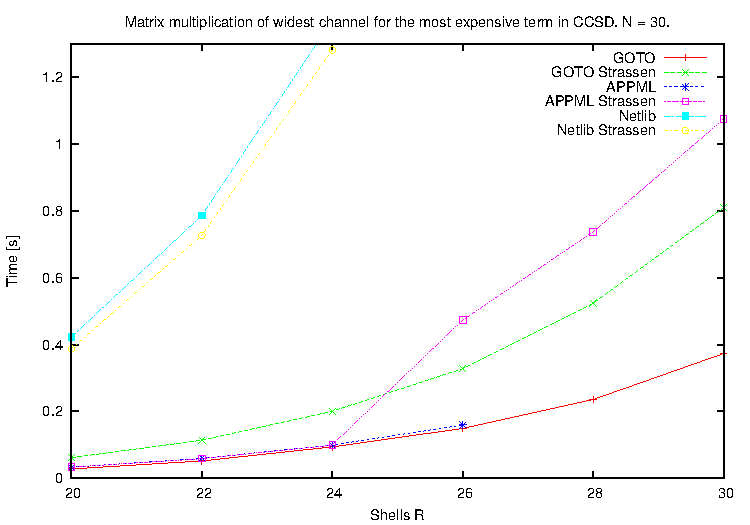
\includegraphics[scale=0.6]{../10-results/figs/timeMult/timeMultCC_5.pdf}
}
\subfigure[$N=56$]{
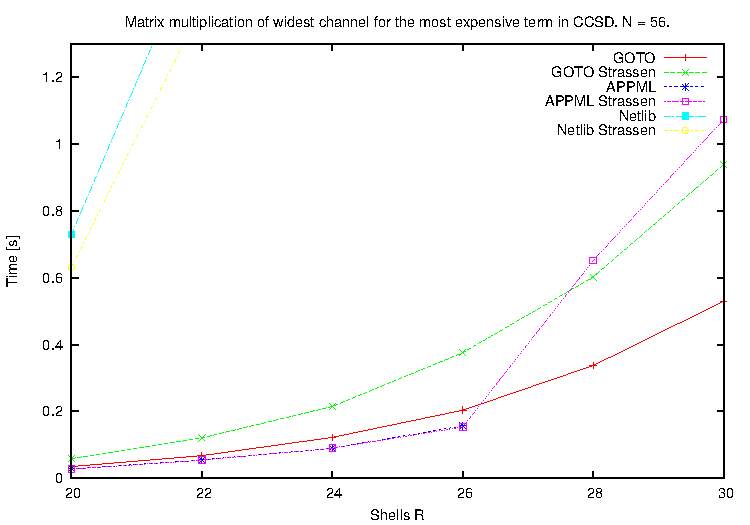
\includegraphics[scale=0.6]{../10-results/figs/timeMult/timeMultCC_7.pdf}
}
\caption{Time usage computing the widest channel in the most expensive term from coupled-cluster $\hat{T}_2$ equations.}
\label{fig:results:timeMultCC}
\end{center}
\end{figure}

With one filled shell, two electrons, we see clearly disadvantages of using GPU's or Strassen's method.
The right matrix is no more than two elements wide, making it unsuitable for such a massive parallelization or further splitting.
Also seen is a dramatic amount of overhead performing the Strassen splitting after the GPU runs out of memory at 26 shells.

Increasing the number of particles, the right matrix will widen slightly, ending at $144$ elements wide for $N=56$.
Still a fairly thin matrix, neither Strassen nor GPU implementations can hold up against Goto's implementation, known to perform well in parallel over shared memory.
Compared to Netlib's reference implementation, now more than ten times slower and barely included in the figure, parallel implementations prove their usefulness.




\paragraph{}
The results from the coupled-cluster benchmarks do not point toward any gain by using GPU's.
In fact the coupled-cluster equations is not the computational bottleneck, compared to the transformation into a Hartree-Fock basis which scales as $ \max_{\lambda}\dim(\xi)^3$ when multiplying two square matrices of size $\dim(\xi)$.

In fig.~\ref{fig:results:timeMultHFsys} the time used to multiply two random matrices whose size matches the largest matrices appearing in the HF-basis transformation.
Now the power of exploiting graphic cards emerges, the APPML implementation being approximately 4 times faster than Goto blas.
Unfortunately we once again see how unfavorable it is to apply a Strassen splitting to prevent running out of memory on the GPU.
After such a splitting our GPU implementation runs at most twice as fast as Goto blas.
\begin{figure}
\begin{center}
\subfigure[$N=2$]{
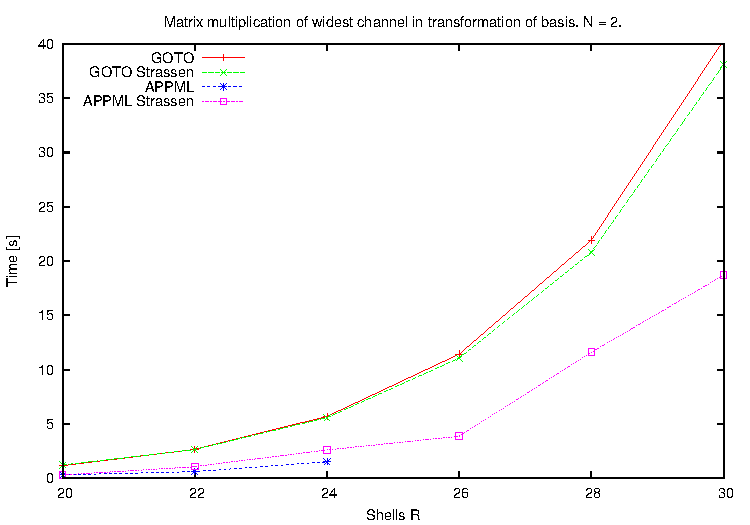
\includegraphics[scale=0.6]{../10-results/figs/timeMult/timeMultHFsys_1.pdf}
}
\subfigure[$N=12$]{
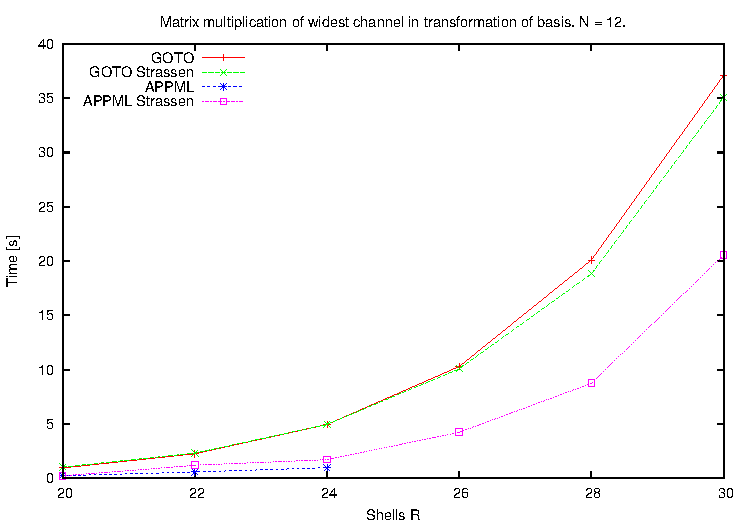
\includegraphics[scale=0.6]{../10-results/figs/timeMult/timeMultHFsys_3.pdf}
}
\subfigure[$N=30$]{
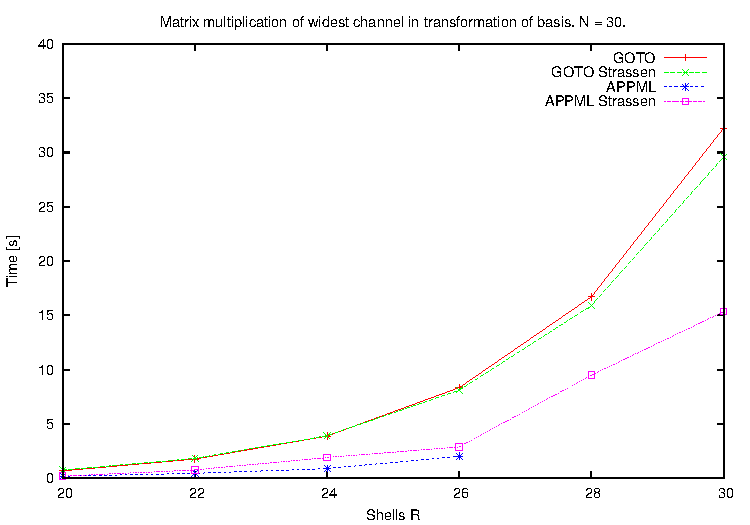
\includegraphics[scale=0.6]{../10-results/figs/timeMult/timeMultHFsys_5.pdf}
}
\subfigure[$N=56$]{
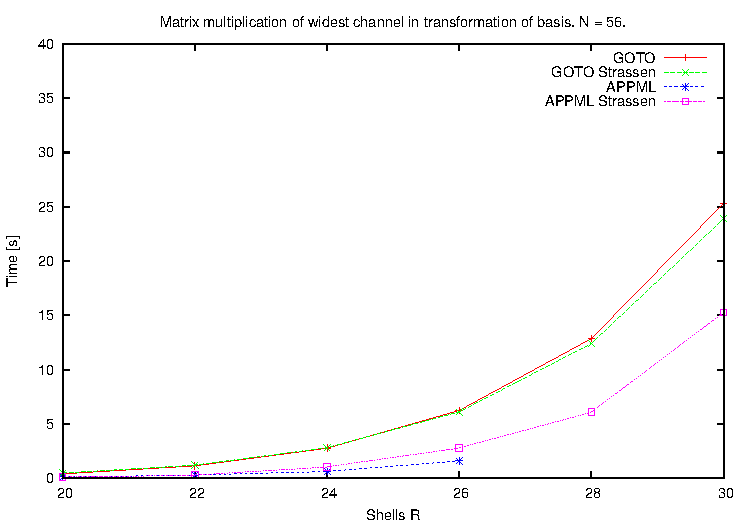
\includegraphics[scale=0.6]{../10-results/figs/timeMult/timeMultHFsys_7.pdf}
}
\caption{Time usage computing the widest channel in the transformation to a Hartree-Fock basis.}
\label{fig:results:timeMultHFsys}
\end{center}
\end{figure}

\paragraph{}
An important aspect regarding both fig.~\ref{fig:results:timeMultCC} and~\ref{fig:results:timeMultHFsys} is that only one Strassen recursion is applied for the Strassen implementations.
For the narrow matrices in the amplitude equations one level of Strassen proved a significant slow down, but shows a small gain when it comes to square matrices.
Table~\ref{tab:results:timeGotoStrassen} shows the time usage comparing the time used by Goto with different levels of Strassen for the large square matrices encountered for 2 electrons in 30 shells.
One, or at most two, levels of recursion is advantageous, not even gaining the theoretical speedup of $12.5\%$.
Our initial tests was using Netlib blas and showed a remarkable improvement, see table~\ref{tab:results:timeNetlibStrassen}, effectively reducing the time consumption of almost $50\%$.
\begin{table}
\begin{center}
\caption{Time used by Goto's and Netlib's blas multiplying two square matrices, for different levels of Strassen splitting.}
\subtable[\label{tab:results:timeGotoStrassen}GOTO blas, matrix size $9412 \times 9412$.]{
\begin{tabular}{c|c|r}
Level & Time [s] & Size \\
\hline
0 & 40.04 & 9412 \\
1 & 37.54 & 4706 \\
2 & 37.42 & 2353 \\
3 & 46.45 & 1176 \\
4 & 52.18 &  588
\end{tabular}
}
\hspace{20mm}
\subtable[\label{tab:results:timeNetlibStrassen}Netlib blas, matrix size $3764 \times 3764$.]{
\begin{tabular}{c|c|r}
Level & Time [s] & Size \\
\hline
0 & 68.31 & 3764 \\
1 & 63.07 & 1882 \\
2 & 47.09 &  941 \\
3 & 41.58 &  470 \\
4 & 40.02 &  235 \\
5 & 39.85 &  117 \\
6 & 35.42 &   58 \\
7 & 36.36 &   29 \\
8 & 53.55 &   14 
\end{tabular}
}
\end{center}
\end{table}




\subsection{Other implementations}
The first Master's project on the topic of writing a C++ coupled-cluster program was completed in 2010 by M. P. Lohne~\cite{mplohne}.
His thesis involved a C++ library looping through all sums over elements stored in Blitz++ arrays.
Elemental access through a linear-algebra library, such as Blitz++, proves inefficient but has the advantage of freeing the programmer of complications and bugs from memory-management.
Lohne, who reached calculations up to 20 electrons and 10 shells, mentions how his code is neither optimized nor parallelized, but still he laid the ground stone for such a study, and concluded his thesis with a remark how future work may include more than 50 electrons in probably 16-20 shells.

M. H. Jørgensen~\cite{marte} continued by optimizing Lohne's library, partly in collaboration with Y. M. Wang~\cite{ymwang}\footnote{Jørgensen and Wang collaborated on optimizing a shared code base, but Wang studied a slightly different system.}.
Their optimizations consisted mainly of replacing Blitz++ constructs with raw pointer syntax and employing a block-diagonal representation for the toughest parts of the interactions.
An example of how successful the optimizations were is mentioned for 12 particles in a basis of 10 major oscillator shells.
Here Lohne's program ran for 35 hours compared to the optimized library now using approximately 4 minutes 30 seconds.

At the beginning of this thesis a decision was made to redesign the entire program to fit a different coding style.
A linear-algebra library was reintroduced, this time Armadillo~\cite{armadillo}, and a more aggressive object orientation was conducted.
Stronger encapsulation was implemented, resulting in fewer classes and cleaner syntax without loosing the flexibility.
Different systems now actually follows a hierarchy, and we have successfully decoupled matrix multiplications from the program as its own module (class).
Timing and debugging is also included, available by invoking simple switches or similar, although turned off by default.

We have compared the time consumption for a few runs in table~\ref{tab:results:timeMarteYangVSme}.
The run case of 12 particles in 10 shells now uses less than four seconds, 35000 times faster than the 35 hours Lohne's implementation used.
Compared with the optimized code of Jørgensen and Wang we see 3-4 times speedup for two particles, more than 20 times for six particles, and roughly 100 times speedup for twelve electrons.
Important here is how the speedup improves for increasing number of particles, a consequence of reducing the dimensionality of all expressions in terms of channels and configurations.
\begin{table}
\begin{center}
\caption{Time}
\label{tab:results:timeMarteYangVSme}
\subtable[$N=2$]{
\begin{tabular}{c||rr|r}
R & Prev & Cur & Factor\\
\hline
10 & 2.9 & 0.9 & 3.2 \\
12 & 8.9 & 2.5 & 3.6 \\
14 & 25  & 6.4 & 3.9 \\
16 & 1:01 & 15 & 4.1 \\
18 & 2:12 & 33 & 4.0 \\
\hline
\end{tabular}
}
\hspace{5mm}
\subtable[$N=6$]{
\begin{tabular}{c||rr|r}
R & Prev & Cur & Factor\\
\hline
10 & 27 & 1.4 & 19 \\
12 & 1:24 & 3.4 & 25 \\
14 & 3:29 & 8.8 & 24 \\
16 & 7:11 & 19 & 23 \\
18 & 16:45 & 43 & 23 \\
\hline
\end{tabular}
}
\subtable[$N=12$]{
\begin{tabular}{c||rr|r}
R & Prev & Cur & Factor\\
\hline
10 & 5:13 & 3.6 & 87 \\
12 & 17:45 & 9.1 & 117 \\
14 &  	NA  &  19 & NA \\
16 &    NA  &  39 & NA \\
18 &    NA  &  1:13 & NA \\
\hline
\end{tabular}
}
\end{center}
\end{table}


In table~\ref{tab:results:timeDissected} we have dissected the time our program uses in the different parts.
\begin{table}
\begin{center}
\caption{What uses the most time?}
\label{tab:results:timeDissected}
\subtable[$N=20$, $R=20$, $\omega = 1.0$]{
\begin{tabular}{l|rr}
Part & Time [s] & $\%$ \\
\hline
Create system \& read file & 36.43~ & 15.6\%~ \\
Hartree-Fock calculation & 20.43~ & 8.7\%~ \\
Hartree-Fock basis & 99.93~ & 42.7\%~ \\
(Spent in matrix multiplication) & (79.39) & (33.9\%)\\
Coupled cluster calculation & 76.98~ & 32.9\%~  \\
(Spent in matrix multiplication) & (24.29) & (10.4\%) \\
\hline 
Total  & 234.05~ & 100.0\%~ \\
\hline \hline
\end{tabular}
}
\\
\vspace{5mm}
\subtable[$N=56$, $R=30$, $\omega = 5.0$]{
\begin{tabular}{l|rr}
Part & Time [s] & $\%$ \\
\hline
Create system \& read file & 928~  &  9.7\%~ \\
Hartree-Fock calculation & 449~ & 4.7\%~ \\
Hartree-Fock basis & 5894~ & 61.7\%~ \\
(Spent in matrix multiplication) & (5034) & (52.7\%)\\
Coupled cluster calculation & 2281~ &  23.9\%~  \\
(Spent in matrix multiplication) & (897) & (9.4\%) \\
\hline 
Total  & 9556~ &  100.0\%~ \\
\hline \hline
\end{tabular}
}
\end{center}
\end{table}

The CC part is dissected even further in table~\ref{tab:results:timeCCdissected}, showing the five most time-consuming parts of the CC machinery.
\begin{table}
\caption{Thoughest terms in CCSD.}
\label{tab:results:timeCCdissected}
\begin{center}
\subtable[$N=20$, $R=20$, $\omega = 1.0$.]{
\begin{tabular}{c|c}
Part & Time [s] \\
\hline
map & 19.9 \\
i11\#2 & 17.5 \\
t2\#2 & 9.4 \\
t2\#8 & 4.8 \\
i10 &  3.7 \\
\hline \hline
\end{tabular}
}
\hspace{5mm}
\subtable[$N=56$, $R=30$, $\omega = 5.0$.]{
\begin{tabular}{c|c}
Part & Time [s] \\
\hline
i11\#2 & 656 \\
map & 455 \\
t2\#2 & 329 \\
i10 & 152 \\
t2\#8 & 140 \\
\hline \hline
\end{tabular}
}
\end{center}
\end{table}




\section{Convergence analysis}
To be able to give a good estimate of the ground state energy we study how the energy converge as a function of the basis.
Including higher shells will contribute less to the ground state energy than lower shells.
If increasing the basis from $R$ to $R+1$ shells alters the energy by an amount $\Delta_{R} E_0$, further increasing the basis will alter the energy by a smaller amount, i.e.
\begin{equation}
\Delta_{R+1} E_0 < \Delta_{R} E_0 .
\end{equation}
It is also believed that including triple excitations contributes less than double excitations, and so on, now yielding a framework to estimate how close we get to the real solution, to be obtained by full configuration interaction (FCI).
FCI includes all possible excitations, finding the eigenvalues of the full Hamiltonian.
For $N$ particles distributed in $n$ states the Hilbert space has a dimensionality
\begin{equation}
\dim(\mathcal{H}) = 
\begin{pmatrix}
n \\ 
N
\end{pmatrix} .
\end{equation}
As an example 6 electrons distributed in 10 oscillator shell, we have $n=110$, resulting in $\sim 2.1 \cdot 10^9$ possible determinants, probably already a challenge to FCI solvers.
For the largest system run here, we have 56 electrons and 30 oscillator shells, equivalent to $930$ basis functions, yielding an enormous amount of $\sim 4.5 \cdot 10^{90}$ combinations. 
In this sense FCI calculations are restricted to a very limited basis size, although including all possible excitations.
CC on the other hand allows a large basis size, but serves equations that are hard to derive and implement already for triples.
For this reason, CC codes for quadruples or higher are seldom seen.

\paragraph{}
We label the energy obtained in a basis of $R$ oscillator shells $E_{M}^{R}$, where $M$ is the method used, either CCSD or HF.
In order to study the convergence properties we define the relative difference in the energy at a specific number of shells to be,
\begin{equation}
\epsilon_M^R = \left| \frac{E_M^R - E_M^{R-2}}{E_M^{R_{\textrm{max}}}}  \right| , 
\end{equation}
in practice the number of significant figures the energy has converged to.

\paragraph{}
For two, six and twelve particles with $\omega = 1.0$ this measure of convergence is visualized in fig.~\ref{fig:results:convN2OM1}.
With few particles and a strong potential convergence is seen to be obtained quickly for the HF energy, fully converged for more than 10 shells, using the standard interaction.
Only the standard interaction sees such a good convergence for the HF energy, as using $V_{\textrm{eff}}$ the energy is still altered by the fourth figure for 24 shells, i.e. $\epsilon^{24}_{HF} >  10^{-4}$.
The CCSD energy, however, converges rapidly for an effective interaction to under $5\cdot 10^{-5}$ before 16 shells, not reached for the standard interaction before $28\sim 30$ shells.
\begin{figure}
\begin{center}
\subfigure[HF]{
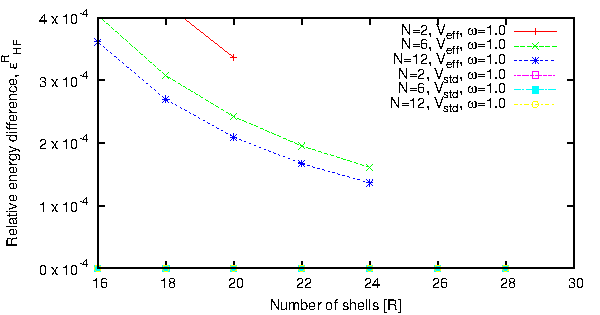
\includegraphics[scale=0.75]{../10-results/figs/convergence/convergencePlotHF_F123_om1_half.pdf}
}
\subfigure[CCSD]{
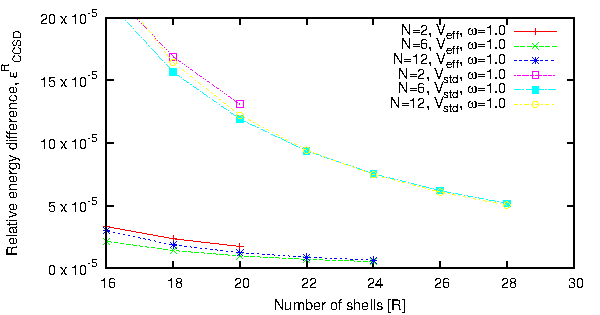
\includegraphics[scale=0.75]{../10-results/figs/convergence/convergencePlotCCSD_F123_om1_half.pdf}
}
\caption{Relative convergence for $N=2$, $6$ and $12$ for $\omega =1.0$.}
\label{fig:results:convN2OM1}
\end{center}
\end{figure}

Raising the number of particles, now for 20, 30 and 42 electrons in fig.~\ref{fig:results:convN20OM1}, we see the same pattern.
The Hartree-Fock energy is fully converged when reaching $R=20$ using the standard interaction, still the effective interaction holds $\epsilon^{24}_{HF} >  10^{-4}$.
The CCSD energy also behaves similar to the case with few particles, although converging slightly slower.
It is remarkable to see how well coupled cluster performs for up to 42 particles, with an error, respective to the basis size, to the fifth significant number.
\begin{figure}
\begin{center}
\subfigure[HF]{
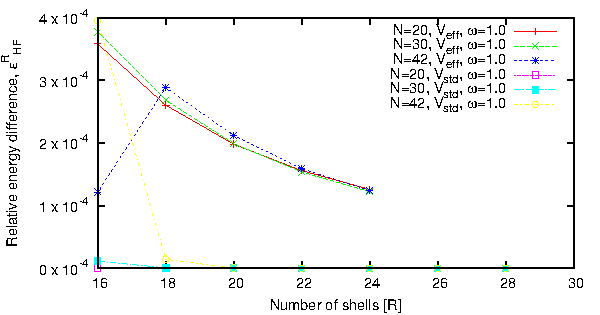
\includegraphics[scale=0.75]{../10-results/figs/convergence/convergencePlotHF_F456_om1_half.pdf}
}
\subfigure[CCSD]{
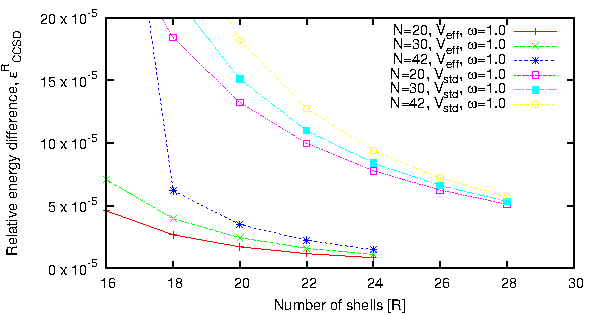
\includegraphics[scale=0.75]{../10-results/figs/convergence/convergencePlotCCSD_F456_om1_half.pdf}
}
\caption{Relative convergence for $N=20$, $30$ and $42$ for $\omega =1.0$.}
\label{fig:results:convN20OM1}
\end{center}
\end{figure}


When the frequency drops to $\omega = 0.1$, as in fig.~\ref{fig:results:convN2OM01}, we see the same tendency in the Hartree-Fock energy, fully converged for the standard interaction, and slightly slower convergence for the effective.
Furthermore we observe that the effective interaction no longer leads to an improvement in convergence.
Except for the two-particle case, where an effective interaction yields the correct result anyhow, both approaches follow similar curves.
Compared to a strongly confined system an effective interaction now performs worse and the standard interaction slightly better.
\begin{figure}
\begin{center}
\subfigure[HF]{
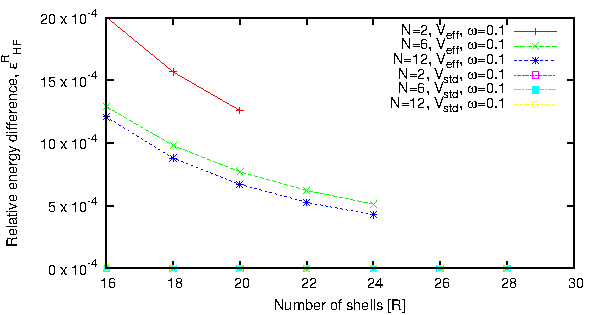
\includegraphics[scale=0.75]{../10-results/figs/convergence/convergencePlotHF_F123_om01_half.pdf}
}
\subfigure[CCSD]{
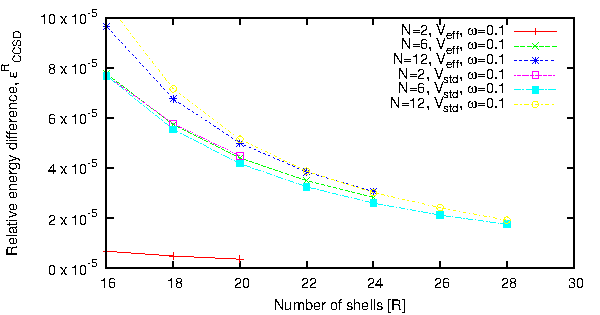
\includegraphics[scale=0.75]{../10-results/figs/convergence/convergencePlotCCSD_F123_om01_half.pdf}
}
\caption{Relative convergence for $N=2$, $6$ and $12$ for $\omega =0.1$.}
\label{fig:results:convN2OM01}
\end{center}
\end{figure}


The last case we study is $N=20$, $30$ and $42$ with a confinement strength of $\omega = 0.7$, the lowest strength that still converges for $42$ electrons, albeit being far from the convergence limit of $N=20$.
The convergence looks consistent with the other strongly confined examples, approaching the same level of convergence for $R_{max}$ although the slope appears to be somewhat steeper.
\begin{figure}
\begin{center}
\subfigure[HF]{
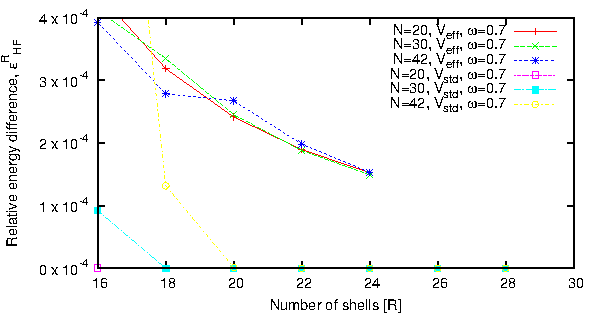
\includegraphics[scale=0.75]{../10-results/figs/convergence/convergencePlotHF_F456_om07_half.pdf}
}
\subfigure[CCSD]{
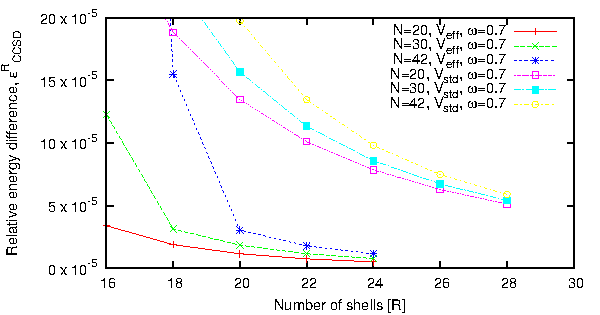
\includegraphics[scale=0.75]{../10-results/figs/convergence/convergencePlotCCSD_F456_om07_half.pdf}
}
\caption{Relative convergence for $N=20$, $30$ and $42$ for $\omega =0.7$.}
\end{center}
\end{figure}


\section{Lowering the frequency}
In order to be able to reach the low oscillator frequencies, down to $0.2$ or lower for systems with less than 20 electrons and $\omega \leq 1.0$ for larger systems, we need to apply a new strategy for the initial guess in the iterative schemes.
No longer can we set the coefficient matrix in Hartree-Fock, $C$, to zero, nor the coupled-cluster amplitudes, $t_i^a$ and $t_{ij}^{ab}$.
In principle these values can be set to anything, and we get the energy eigenvalue of one state, if converging.
Although such a procedure may succeed, it has one major flaw.
Having zero as a first guess reproduces the reference Slater determinant, the exact ground state for a non-interacting system.
Considering an interacting system to be not too different from the uncorrelated, we assume the method to converge toward the ground state.
Other values, if not carefully selected, can converge to other, excited, states.

For a tightly bound system we see no convergence issues, say for a strong potential $\omega = \omega_1$.
The system is now determined mostly by the large single-particle contribution, leaving correlations to determine only a fraction of the total energy.
Our zero-based guess for the coefficients now holds sufficient, and after a number of iterations we find an energy of $E_0(\omega_1)$ as well as coefficients $C(\omega_1)$, $t_i^a(\omega_1)$ and $t_{ij}^{ab}(\omega_1)$.
We claim that both the energy and the coefficients vary only by a small amount  whenever the frequency is also varied by a small change, $\Delta_{\omega}$, i.e.
\begin{equation}
\label{eq:results:omegaStep}
\omega_2 \equiv \omega_1 - \Delta_{\omega} \rightarrow 0 
\Rightarrow 
\left\lbrace
\begin{matrix}
| C(\omega_1) - C(\omega_2) | \rightarrow 0 , \vspace{1mm}\\
| t_i^a(\omega_1) - t_i^a(\omega_2) | \rightarrow 0 ,\vspace{1mm}\\
| t_{ij}^{ab}(\omega) - t_{ij}^{ab}(\omega_2) | \rightarrow 0 ,\vspace{1mm}\\
| E_0(\omega_1) - E_0(\omega_2) | \rightarrow 0 .
\end{matrix}
\right.
\end{equation}
Although~\eqref{eq:results:omegaStep} is left unproven here, we see clearly such a behavior in practice.

Applied iteratively, we now store coefficients from one run, lower the frequency, then calculate the new coefficients and energy, taking the stored coefficients as initial values.
Allowing us to reach previously unavailable frequencies, this technique also increases the CPU time by the amount of intermediate $\omega$ values needed.
It is believed that we could push the lower level somewhat further, taking smaller intermediate steps, but time constraints prevented us from doing so in this thesis.


\paragraph{}
In order to study the role of correlations for different number of particles and a varying omega, we define the relative correlation energy
\begin{equation}
\label{eq:results:relCorr}
\chi = \left|  \frac{E_{CCSD} - \langle \hat{H}_0 \rangle}{E_{CCSD}}  \right| ,
\end{equation}
where $\langle \hat{H}_0 \rangle $ is the energy of an uncorrelated system. 
Uncorrelated energies for specific values of $N$ and $\omega$ can be found in table~\ref{tab:results:Euncorr}.
We naturally expect the two limits
\begin{equation}
\lim_{\omega \rightarrow 0} \chi = 1,
\textrm{ and }
\lim_{\omega \rightarrow \infty} \chi = 0,
\end{equation}
as a tightly bound system is dominated by the high single-particle energy, and as $\omega$ tends to zero we obtain a free electron-gas with no potential and all energy a consequence of correlations.
The results for $\chi$ are shown in fig.~\ref{fig:results:relCorr}.
From this figure we see that interactions are increasingly important when the oscillator frequency is lowered.
Furthermore, we see an increase in correlations whenever more particles are added to the system.
\begin{figure}
\begin{center}
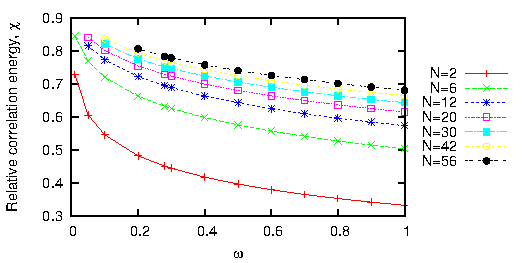
\includegraphics[scale=1.4]{../10-results/figs/loweringOmega/correlationAllZoom.pdf}
\caption{Relative correlation energy}
\label{fig:results:relCorr}
\end{center}
\end{figure}


Also studied are correlations with respect to the Hartree-Fock, defined similar to \eqref{eq:results:relCorr},
\begin{equation}
\label{eq:results:relCorrHF}
\Xi = \left| \frac{E_{CCSD} - E_{HF} }{E_{CCSD}} \right| .
\end{equation}
If we recall how the Hartree-Fock method treats a many-body system as an uncorrelated system, only transforming the single-particle basis, we can interpret HF as solving an uncorrelated system where each electron is subjected to a mean field set up by the other electrons.
\begin{figure}
\begin{center}
\subfigure[FEW Particles :D]{
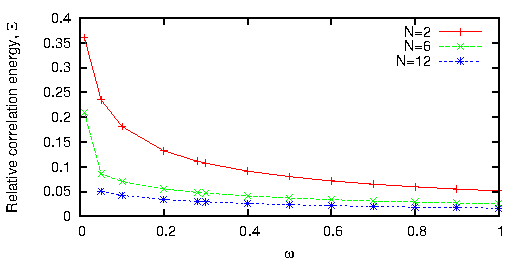
\includegraphics[scale=0.85]{../10-results/figs/loweringOmega/correlationMeanField_2_6_12_Zoom.pdf}
}
\subfigure[MANY Particles :D]{
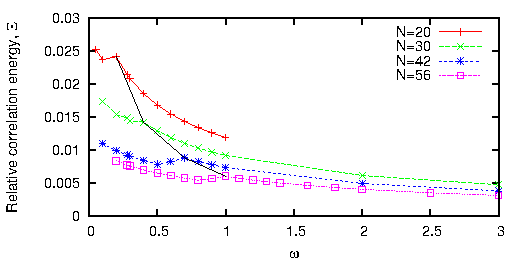
\includegraphics[scale=0.85]{../10-results/figs/loweringOmega/correlationMeanField_20_30_42_56_Zoom.pdf}
}
\caption{Relative correlation energy with respect to the mean-field approximation, $E_{HF}$.}
\label{fig:results:relCorrHF}
\end{center}
\end{figure}


\section{Comparison with other methods}
\subsection{Variational Monte Carlo}
\subsection{Diffusion Monte Carlo}
\subsection{Full configuration interaction}


\FloatBarrier
\section{Tables}
\label{sec:results:theResults}
\subsection{Harmonic-oscillator basis}
\FloatBarrier

\begin{table}
\begin{center}
Standard interaction, $F=1$, HO basis.\\
\begin{tabular}{l|rrrrrr}
\hline 
$E_{CCSD}$ & 10 & 12 & 14 & 16 & 18 & 20 \\
\hline \hline
1.0 & 3.0069 & 3.0055 & 3.0046 & 3.0039 & 3.0034 & 3.0030  \\ 
0.9 & 2.7459 & 2.7446 & 2.7437 & 2.7431 & 2.7426 & 2.7423  \\ 
0.8 & 2.4817 & 2.4805 & 2.4797 & 2.4792 & 2.4788 & 2.4784  \\ 
0.7 & 2.2138 & 2.2128 & 2.2120 & 2.2115 & 2.2112 & 2.2109  \\ 
0.6 & 1.9414 & 1.9405 & 1.9399 & 1.9395 & 1.9391 & 1.9389  \\ 
0.5 & 1.6635 & 1.6628 & 1.6622 & 1.6619 & 1.6616 & 1.6614  \\ 
0.4 & 1.3785 & 1.3779 & 1.3775 & 1.3772 & 1.3770 & 1.3769  \\ 
0.3 & 1.0840 & 1.0835 & 1.0832 & 1.0830 & 1.0829 & 1.0828  \\ 
0.28 & 1.0236 & 1.0232 & 1.0229 & 1.0227 & 1.0226 & 1.0225  \\ 
0.2 & 0.7752 & 0.7749 & 0.7747 & 0.7746 & 0.7745 & 0.7745  \\ 
0.1 & 0.4411 & 0.4411 & 0.4410 & 0.4410 & 0.4410 & 0.4409  \\ 
0.05 & 0.2541 & 0.2541 & 0.2541 & 0.2541 & 0.2541 & 0.2541  \\ 
0.01 & DNC & DNC & 0.5781 & 0.6304 & DNC & DNC  \\ 
\hline \hline
\end{tabular}
\end{center}
\end{table}

\begin{table}
\begin{center}
Effective interaction, $F=1$, HO basis.\\
\begin{tabular}{l|rrrrrr}
\hline 
$E_{CCSD}$ & 10 & 12 & 14 & 16 & 18 & 20 \\
\hline \hline
1.0 & 3.0009 & 3.0007 & 3.0005 & 3.0004 & 3.0003 & 3.0003  \\ 
0.9 & 2.7403 & 2.7401 & 2.7400 & 2.7399 & 2.7398 & 2.7398  \\ 
0.8 & 2.4766 & 2.4764 & 2.4763 & 2.4762 & 2.4762 & 2.4761  \\ 
0.7 & 2.2093 & 2.2091 & 2.2090 & 2.2089 & 2.2089 & 2.2088  \\ 
0.6 & 1.9375 & 1.9373 & 1.9372 & 1.9372 & 1.9371 & 1.9371  \\ 
0.5 & 1.6602 & 1.6601 & 1.6600 & 1.6600 & 1.6599 & 1.6599  \\ 
0.4 & 1.3759 & 1.3758 & 1.3758 & 1.3757 & 1.3757 & 1.3757  \\ 
0.3 & 1.0821 & 1.0820 & 1.0820 & 1.0820 & 1.0820 & 1.0819  \\ 
0.28 & 1.0218 & 1.0218 & 1.0218 & 1.0217 & 1.0217 & 1.0217  \\ 
0.2 & 0.7741 & 0.7741 & 0.7740 & 0.7740 & 0.7740 & 0.7740  \\ 
0.1 & 0.4408 & 0.4408 & 0.4408 & 0.4408 & 0.4408 & 0.4408  \\ 
0.05 & 0.2541 & 0.2541 & 0.2541 & 0.2541 & 0.2541 & 0.2541  \\ 
0.01 & 0.0738 & 0.0738 & 0.0738 & 0.0738 & 0.0738 & 0.0738  \\ 
\hline \hline
\end{tabular}
\end{center}
\end{table}

\begin{table}
\begin{center}
Standard interaction, $F=2$, HO basis.\\
\begin{tabular}{l|rrrrrr}
\hline 
$E_{CCSD}$ & 10 & 12 & 14 & 16 & 18 & 20 \\
\hline \hline
1.0 & 20.2043 & 20.1947 & 20.1885 & 20.1843 & 20.1812 & 20.1789  \\ 
0.9 & 18.6033 & 18.5944 & 18.5887 & 18.5848 & 18.5819 & 18.5798  \\ 
0.8 & 16.9703 & 16.9621 & 16.9570 & 16.9534 & 16.9508 & 16.9488  \\ 
0.7 & 15.2995 & 15.2922 & 15.2876 & 15.2844 & 15.2821 & 15.2803  \\ 
0.6 & 13.5830 & 13.5767 & 13.5727 & 13.5699 & 13.5679 & 13.5664  \\ 
0.5 & 11.8098 & 11.8045 & 11.8011 & 11.7988 & 11.7971 & 11.7958  \\ 
0.4 & 9.9630 & 9.9588 & 9.9562 & 9.9543 & 9.9530 & 9.9520  \\ 
0.3 & 8.0154 & 8.0125 & 8.0106 & 8.0093 & 8.0084 & 8.0077  \\ 
0.28 & 7.6100 & 7.6073 & 7.6056 & 7.6044 & 7.6036 & 7.6030  \\ 
0.2 & 5.9158 & 5.9142 & 5.9131 & 5.9124 & 5.9119 & 5.9115  \\ 
0.1 & 3.5398 & 3.5394 & 3.5392 & DNC & DNC & DNC  \\ 
0.05 & 1.9742 & DNC & DNC  \\ 
0.01 & DNC  \\ 
\hline \hline
\end{tabular}
\end{center}
\end{table}

\begin{table}
\begin{center}
Effective interaction, $F=2$, HO basis.\\
\begin{tabular}{l|rrrrrr}
\hline 
$E_{CCSD}$ & 10 & 12 & 14 & 16 & 18 & 20 \\
\hline \hline
1.0 & 20.1660 & 20.1646 & 20.1639 & 20.1634 & 20.1631 & 20.1629  \\ 
0.9 & 18.5676 & 18.5664 & 18.5658 & 18.5654 & 18.5652 & 18.5650  \\ 
0.8 & 16.9375 & 16.9365 & 16.9360 & 16.9357 & 16.9355 & 16.9353  \\ 
0.7 & 15.2699 & 15.2691 & 15.2687 & 15.2685 & 15.2683 & 15.2682  \\ 
0.6 & 13.5570 & 13.5564 & 13.5561 & 13.5559 & 13.5558 & 13.5557  \\ 
0.5 & 11.7877 & 11.7873 & 11.7871 & 11.7870 & 11.7869 & 11.7869  \\ 
0.4 & 9.9454 & 9.9452 & 9.9450 & 9.9450 & 9.9449 & 9.9449  \\ 
0.3 & 8.0028 & 8.0027 & 8.0027 & 8.0027 & 8.0027 & 8.0027  \\ 
0.28 & 7.5985 & 7.5984 & 7.5984 & 7.5984 & 7.5984 & 7.5984  \\ 
0.2 & 5.9089 & 5.9089 & 5.9088 & 5.9088 & 5.9088 & 5.9088  \\ 
0.1 & 3.5392 & 3.5390 & 3.5389 & 3.5388 & 3.5388 & 3.5387  \\ 
0.05 & 2.0215 & 2.0152 & 2.0104 & DNC & DNC & DNC  \\ 
0.01 & 0.6119 & 0.6021 & 0.5968  \\ 
\hline \hline
\end{tabular}
\end{center}
\end{table}

\begin{table}
\begin{center}
Standard interaction, $F=3$, HO basis.\\
\begin{tabular}{l|rrrrrr}
\hline 
$E_{CCSD}$ & 10 & 12 & 14 & 16 & 18 & 20 \\
\hline \hline
1.0 & 65.8065 & 65.7673 & 65.7443 & 65.7292 & 65.7186 & 65.7107  \\ 
0.9 & 60.7696 & 60.7330 & 60.7116 & 60.6976 & 60.6878 & 60.6805  \\ 
0.8 & 55.6144 & 55.5806 & 55.5610 & 55.5481 & 55.5391 & 55.5324  \\ 
0.7 & 50.3192 & 50.2886 & 50.2709 & 50.2594 & 50.2513 & 50.2453  \\ 
0.6 & 44.8551 & 44.8281 & 44.8125 & 44.8023 & 44.7952 & 44.7900  \\ 
0.5 & 39.1810 & 39.1580 & 39.1447 & 39.1361 & DNC & DNC  \\ 
0.4 & 33.2355 & 33.2168 & DNC & DNC  \\ 
0.3 & 26.9178 & DNC  \\ 
0.28 & 25.5956  \\ 
0.2 & DNC  \\ 
\hline \hline
\end{tabular}
\end{center}
\end{table}

\begin{table}
\begin{center}
Effective interaction, $F=3$, HO basis.\\
\begin{tabular}{l|rrrrrr}
\hline 
$E_{CCSD}$ & 10 & 12 & 14 & 16 & 18 & 20 \\
\hline \hline
1.0 & 65.6831 & 65.6745 & 65.6700 & 65.6674 & 65.6657 & 65.6645  \\ 
0.9 & 60.6549 & 60.6470 & 60.6429 & 60.6405 & 60.6389 & 60.6378  \\ 
0.8 & 55.5092 & 55.5020 & 55.4983 & 55.4961 & 55.4947 & 55.4937  \\ 
0.7 & 50.2247 & 50.2183 & 50.2150 & 50.2132 & 50.2117 & 50.2108  \\ 
0.6 & 44.7725 & 44.7670 & 44.7640 & 44.7623 & 44.7611 & 44.7603  \\ 
0.5 & 39.1119 & 39.1072 & 39.1046 & 39.1030 & 39.1020 & 39.1013  \\ 
0.4 & 33.1818 & 33.1777 & 33.1754 & 33.1741 & DNC & DNC  \\ 
0.3 & 26.8814 & 26.8782 & DNC & DNC  \\ 
0.28 & 25.5628 & DNC  \\ 
0.2 & DNC  \\ 
\hline \hline
\end{tabular}
\end{center}
\end{table}

\FloatBarrier
\subsection{Hartree-Fock basis}
\FloatBarrier
\begin{landscape}
\begin{table}
\begin{center}
Standard interaction, $F=1$.\\
\begin{tabular}{l|rrrrrrrrrrr}
\hline 
$E_{HF}$ & 10 & 12 & 14 & 16 & 18 & 20 & 22 & 24 & 26 & 28 \\ 
\hline \hline
1.0 & 3.1619 & 3.1619 & 3.1619 & 3.1619 & 3.1619 & 3.1619  \\ 
0.9 & 2.8983 & 2.8983 & 2.8983 & 2.8983 & 2.8983 & 2.8983  \\ 
0.8 & 2.6311 & 2.6311 & 2.6311 & 2.6311 & 2.6311 & 2.6311  \\ 
0.7 & 2.3596 & 2.3596 & 2.3596 & 2.3596 & 2.3596 & 2.3596  \\ 
0.6 & 2.0829 & 2.0829 & 2.0829 & 2.0829 & 2.0829 & 2.0829  \\ 
0.5 & 1.7997 & 1.7997 & 1.7997 & 1.7997 & 1.7997 & 1.7997  \\ 
0.4 & 1.5080 & 1.5080 & 1.5080 & 1.5080 & 1.5080 & 1.5080  \\ 
0.3 & 1.2044 & 1.2044 & 1.2044 & 1.2044 & 1.2044 & 1.2044  \\ 
0.28 & 1.1417 & 1.1417 & 1.1417 & 1.1417 & 1.1417 & 1.1417  \\ 
0.2 & 0.8823 & 0.8823 & 0.8823 & 0.8823 & 0.8823 & 0.8823  \\ 
0.1 & 0.5256 & 0.5256 & 0.5256 & 0.5256 & 0.5256 & 0.5256  \\ 
0.05 & 0.3178 & 0.3178 & 0.3178 & 0.3178 & 0.3178 & 0.3178  \\ 
0.01 & 0.1028 & 0.1028 & 0.1028 & 0.1028 & 0.1028 & 0.1028  \\ 
\hline \hline
\end{tabular} 
\end{center}
\begin{center}
Standard interaction, $F=1$, HF basis.\\
\begin{tabular}{l|rrrrrrrrrr}
\hline 
$E_{CCSD}$ & 10 & 12 & 14 & 16 & 18 & 20 & 22 & 24 & 26 & 28 \\
\hline \hline
1.0 & 3.0069 & 3.0055 & 3.0046 & 3.0039 & 3.0034 & 3.0030  \\ 
0.9 & 2.7459 & 2.7446 & 2.7437 & 2.7431 & 2.7426 & 2.7423  \\ 
0.8 & 2.4817 & 2.4805 & 2.4797 & 2.4792 & 2.4788 & 2.4784  \\ 
0.7 & 2.2138 & 2.2128 & 2.2120 & 2.2115 & 2.2112 & 2.2109  \\ 
0.6 & 1.9414 & 1.9405 & 1.9399 & 1.9395 & 1.9391 & 1.9389  \\ 
0.5 & 1.6635 & 1.6628 & 1.6622 & 1.6619 & 1.6616 & 1.6614  \\ 
0.4 & 1.3785 & 1.3779 & 1.3775 & 1.3772 & 1.3770 & 1.3769  \\ 
0.3 & 1.0840 & 1.0835 & 1.0832 & 1.0830 & 1.0829 & 1.0828  \\ 
0.28 & 1.0236 & 1.0232 & 1.0229 & 1.0227 & 1.0226 & 1.0225  \\ 
0.2 & 0.7752 & 0.7749 & 0.7747 & 0.7746 & 0.7745 & 0.7745  \\ 
0.1 & 0.4411 & 0.4411 & 0.4410 & 0.4410 & 0.4410 & 0.4409  \\ 
0.05 & 0.2541 & 0.2541 & 0.2541 & 0.2541 & 0.2541 & 0.2541  \\ 
0.01 & 0.0738 & 0.0738 & 0.0738 & 0.6304 & DNC & DNC  \\
\hline \hline
\end{tabular}
\end{center}
\end{table}
\end{landscape}


 
\begin{landscape}
\begin{table}
\begin{center}
Effective interaction, $F=1$.\\
\begin{tabular}{l|rrrrrrrrr}
\hline 
$E_{HF}$ & 10 & 12 & 14 & 16 & 18 & 20 & 22 & 24\\ 
\hline \hline
1.0 & 3.1429 & 3.1461 & 3.1484 & 3.1501 & 3.1514 & 3.1525  \\ 
0.9 & 2.8795 & 2.8827 & 2.8849 & 2.8866 & 2.8879 & 2.8890  \\ 
0.8 & 2.6126 & 2.6157 & 2.6179 & 2.6196 & 2.6209 & 2.6219  \\ 
0.7 & 2.3415 & 2.3445 & 2.3467 & 2.3483 & 2.3496 & 2.3506  \\ 
0.6 & 2.0653 & 2.0682 & 2.0703 & 2.0719 & 2.0732 & 2.0741  \\ 
0.5 & 1.7826 & 1.7855 & 1.7875 & 1.7891 & 1.7903 & 1.7912  \\ 
0.4 & 1.4916 & 1.4943 & 1.4963 & 1.4978 & 1.4989 & 1.4998  \\ 
0.3 & 1.1888 & 1.1914 & 1.1933 & 1.1946 & 1.1957 & 1.1966  \\ 
0.28 & 1.1264 & 1.1290 & 1.1308 & 1.1321 & 1.1332 & 1.1341  \\ 
0.2 & 0.8681 & 0.8705 & 0.8721 & 0.8734 & 0.8744 & 0.8752  \\ 
0.1 & 0.5138 & 0.5157 & 0.5171 & 0.5182 & 0.5190 & 0.5196  \\ 
0.05 & 0.3083 & 0.3098 & 0.3109 & 0.3118 & 0.3124 & 0.3129  \\ 
0.01 & 0.0971 & 0.0980 & 0.0987 & 0.0992 & 0.0996 & 0.1000  \\ 
\hline \hline
\end{tabular} 
\end{center}
\begin{center}
Effective interaction, $F=1$, HF basis.\\
\begin{tabular}{l|rrrrrrrr}
\hline 
$E_{CCSD}$ & 10 & 12 & 14 & 16 & 18 & 20 & 22 & 24\\
\hline \hline
1.0 & 3.0009 & 3.0007 & 3.0005 & 3.0004 & 3.0003 & 3.0003  \\ 
0.9 & 2.7403 & 2.7401 & 2.7400 & 2.7399 & 2.7398 & 2.7398  \\ 
0.8 & 2.4766 & 2.4764 & 2.4763 & 2.4762 & 2.4762 & 2.4761  \\ 
0.7 & 2.2093 & 2.2091 & 2.2090 & 2.2089 & 2.2089 & 2.2088  \\ 
0.6 & 1.9375 & 1.9373 & 1.9372 & 1.9372 & 1.9371 & 1.9371  \\ 
0.5 & 1.6602 & 1.6601 & 1.6600 & 1.6600 & 1.6599 & 1.6599  \\ 
0.4 & 1.3759 & 1.3758 & 1.3758 & 1.3757 & 1.3757 & 1.3757  \\ 
0.3 & 1.0821 & 1.0820 & 1.0820 & 1.0820 & 1.0820 & 1.0819  \\ 
0.28 & 1.0218 & 1.0218 & 1.0218 & 1.0217 & 1.0217 & 1.0217  \\ 
0.2 & 0.7741 & 0.7741 & 0.7740 & 0.7740 & 0.7740 & 0.7740  \\ 
0.1 & 0.4408 & 0.4408 & 0.4408 & 0.4408 & 0.4408 & 0.4408  \\ 
0.05 & 0.2541 & 0.2541 & 0.2541 & 0.2541 & 0.2541 & 0.2541  \\ 
0.01 & 0.0738 & 0.0738 & 0.0738 & 0.0738 & 0.0738 & 0.0738  \\ 
\hline \hline
\end{tabular}
\end{center}
\end{table}
\end{landscape}







\begin{landscape}
\begin{table}
\begin{center}
Standard interaction, $F=2$.\\
\begin{tabular}{l|rrrrrrrrrr}
\hline 
$E_{HF}$ & 10 & 12 & 14 & 16 & 18 & 20 & 22 & 24 & 26 & 28 \\
\hline \hline
1.0 & 20.7192 & 20.7192 & 20.7192 & 20.7192 & 20.7192 & 20.7192 & 20.7192 & 20.7192 & 20.7192 & 20.7192 \\ 
0.9 & 19.1108 & 19.1108 & 19.1108 & 19.1108 & 19.1108 & 19.1108 & 19.1108 & 19.1108 & 19.1108 & 19.1108 \\ 
0.8 & 17.4693 & 17.4693 & 17.4693 & 17.4693 & 17.4693 & 17.4693 & 17.4693 & 17.4693 & 17.4693 & 17.4693 \\ 
0.7 & 15.7884 & 15.7883 & 15.7883 & 15.7883 & 15.7883 & 15.7883 & 15.7883 & 15.7883 & 15.7883 & 15.7883 \\ 
0.6 & 14.0597 & 14.0597 & 14.0597 & 14.0597 & 14.0597 & 14.0597 & 14.0597 & 14.0597 & 14.0597 & 14.0597 \\ 
0.5 & 12.2713 & 12.2713 & 12.2713 & 12.2713 & 12.2713 & 12.2713 & 12.2713 & 12.2713 & 12.2713 & 12.2713 \\ 
0.4 & 10.4052 & 10.4052 & 10.4052 & 10.4052 & 10.4052 & 10.4052 & 10.4052 & 10.4052 & 10.4052 & 10.4052 \\ 
0.3 & 8.4314 & 8.4314 & 8.4314 & 8.4314 & 8.4314 & 8.4314       &  8.4314 &  8.4314 &  8.4314 &  8.4314 \\ 
0.28 & 8.0196 & 8.0196 & 8.0196 & 8.0196 & 8.0196 & 8.0196      &  8.0196 &  8.0196 &  8.0196 &  8.0196 \\ 
0.2 & 6.2935 & 6.2935 & 6.2935 & 6.2935 & 6.2935 & 6.2935       &  6.2935 &  6.2935 &  6.2935 &  6.2935 \\ 
0.1 & 3.8524 & 3.8524 & 3.8524 & 3.8524 & 3.8524 & 3.8524       &  3.8524 &  3.8524 &  3.8524 &  3.8524 \\ 
0.05 & 2.3791 & 2.3790 & 2.3790 & 2.3790 & 2.3790 & 2.3790      &  2.3790 &  2.3790 &  2.3790 &  2.3790 \\ 
0.01 & 0.7999 & 0.7947 & 0.7936 & 0.7935 & 0.7935 & 0.7935      &  0.7935 &  0.7935 &  0.7935 &  0.7935 \\ 
\hline \hline
\end{tabular}
\end{center}
\begin{center}
Standard interaction, $F=2$, HF basis.\\
\begin{tabular}{l|rrrrrrrrrr}
\hline 
$E_{CCSD}$ & 10 & 12 & 14 & 16 & 18 & 20 & 22 & 24 & 26 & 28 \\
\hline \hline
1.0 & 20.2161 & 20.2063 & 20.2000 & 20.1957 & 20.1925 & 20.1901 & 20.1882 & 20.1867 & 20.1854 & 20.1844 \\ 
0.9 & 18.6162 & 18.6070 & 18.6012 & 18.5972 & 18.5943 & 18.5921 & 18.5903 & 18.5889 & 18.5877 & 18.5868 \\ 
0.8 & 16.9845 & 16.9761 & 16.9708 & 16.9671 & 16.9645 & 16.9624 & 16.9608 & 16.9596 & 16.9585 & 16.9576 \\ 
0.7 & 15.3153 & 15.3078 & 15.3030 & 15.2997 & 15.2973 & 15.2955 & 15.2940 & 15.2929 & 15.2920 & 15.2912 \\ 
0.6 & 13.6008 & 13.5942 & 13.5900 & 13.5871 & 13.5850 & 13.5834 & 13.5822 & 13.5812 & 13.5804 & 13.5797 \\ 
0.5 & 11.8301 & 11.8245 & 11.8209 & 11.8185 & 11.8167 & 11.8154 & 11.8143 & 11.8135 & 11.8128 & 11.8122 \\ 
0.4 & 9.9866 & 9.9820 & 9.9792 & 9.9773 & 9.9759 & 9.9748       &  9.9739 & 9.9733  &  9.9727 &  9.9723 \\ 
0.3 & 8.0434 & 8.0401 & 8.0380 & 8.0366 & 8.0356 & 8.0348       &  8.0342 & 8.0337  &  8.0333 &  8.0330 \\ 
0.28 & 7.6390 & 7.6360 & 7.6341 & 7.6328 & 7.6319 & 7.6312      &  7.6306 & 7.6302  &  7.6298 &  7.6295 \\ 
0.2 & 5.9501 & 5.9481 & 5.9469 & 5.9460 & 5.9454 & 5.9450       &  5.9446 & 5.9443  &  5.9441 &  5.9439 \\ 
0.1 & 3.5841 & 3.5835 & 3.5831 & 3.5828 & 3.5826 & 3.5825       &  3.5823 & 3.5822  &  3.5822 &  3.5821 \\ 
0.05 & 2.1776 & 2.1775 & 2.1774 & 2.1773 & 2.1773 & 2.1772      &  2.1772 & 2.1772  &  2.1772 &  2.1772 \\ 
0.01 & 0.6267 & 0.6282 & DNC & DNC & DNC & DNC                  &  DNC    & DNC     &  DNC    &     DNC \\ 
\hline \hline
\end{tabular}
\end{center}
\end{table}
\end{landscape}

 
 
\begin{landscape}
\begin{table}
\begin{center}
Effective interaction, $F=2$.\\
\begin{tabular}{l|rrrrrrrr}
\hline 
$E_{HF}$ & 10 & 12 & 14 & 16 & 18 & 20 & 22 & 24 \\
\hline \hline
1.0 & 20.6295 & 20.6461 & 20.6576 & 20.6659 & 20.6723 & 20.6773 & 20.6813  & 20.6847 \\ 
0.9 & 19.0228 & 19.0391 & 19.0503 & 19.0585 & 19.0648 & 19.0697 & 19.0736  & 19.0769 \\ 
0.8 & 17.3831 & 17.3991 & 17.4100 & 17.4181 & 17.4242 & 17.4290 & 17.4329  & 17.4361 \\ 
0.7 & 15.7043 & 15.7199 & 15.7306 & 15.7384 & 15.7444 & 15.7491 & 15.7529  & 15.7560 \\ 
0.6 & 13.9781 & 13.9933 & 14.0037 & 14.0112 & 14.0170 & 14.0216 & 14.0253  & 14.0283 \\ 
0.5 & 12.1927 & 12.2073 & 12.2173 & 12.2246 & 12.2302 & 12.2346 & 12.2381  & 12.2411 \\ 
0.4 & 10.3302 & 10.3441 & 10.3537 & 10.3606 & 10.3659 & 10.3701 & 10.3735  & 10.3763 \\ 
0.3 &  8.3611 &  8.3741 &  8.3831 &  8.3896 &  8.3946 &  8.3985 &  8.4017  &  8.4043 \\ 
0.28 & 7.9504 &  7.9632 &  7.9720 &  7.9785 &  7.9834 &  7.9872 &  7.9903  &  7.9929 \\ 
0.2 &  6.2297 &  6.2416 &  6.2497 &  6.2556 &  6.2602 &  6.2637 &  6.2666  &  6.2689 \\ 
0.1 &  3.7991 &  3.8091 &  3.8159 &  3.8208 &  3.8246 &  3.8275 &  3.8299  &  3.8319 \\ 
0.05 & 2.3353 &  2.3437 &  2.3493 &  2.3534 &  2.3564 &  2.3589 &  2.3608  &  2.3624 \\ 
0.01 & 0.7659 &  0.7704 &  0.7742 &  0.7772 &  0.7793 &  0.7810 &  0.7823  &  0.7834 \\ 
\hline \hline
\end{tabular}
\end{center}
\begin{center}
Effective interaction, $F=2$, HF basis.\\
\begin{tabular}{l|rrrrrrrr}
\hline 
$E_{CCSD}$ & 10 & 12 & 14 & 16 & 18 & 20 & 22 & 24 \\
\hline \hline
1.0 & 20.1766 & 20.1753 & 20.1746 & 20.1742 & 20.1739 & 20.1737  & 20.1735 & 20.1734 \\ 
0.9 & 18.5792 & 18.5781 & 18.5775 & 18.5771 & 18.5769 & 18.5768  & 18.5766 & 18.5766 \\ 
0.8 & 16.9502 & 16.9494 & 16.9489 & 16.9486 & 16.9484 & 16.9483  & 16.9482 & 16.9482 \\ 
0.7 & 15.2841 & 15.2834 & 15.2831 & 15.2829 & 15.2827 & 15.2827  & 15.2826 & 15.2826 \\ 
0.6 & 13.5729 & 13.5724 & 13.5722 & 13.5721 & 13.5721 & 13.5720  & 13.5720 & 13.5720 \\ 
0.5 & 11.8057 & 11.8055 & 11.8055 & 11.8055 & 11.8055 & 11.8055  & 11.8055 & 11.8055 \\ 
0.4 &  9.9662 &  9.9663 &  9.9664 &  9.9665 &  9.9665 &  9.9666  &  9.9666 &  9.9667 \\ 
0.3 &  8.0275 &  8.0278 &  8.0280 &  8.0282 &  8.0283 &  8.0285  &  8.0285 &  8.0286 \\ 
0.28 & 7.6241 &  7.6245 &  7.6247 &  7.6249 &  7.6251 &  7.6252  &  7.6253 &  7.6254 \\ 
0.2 &  5.9392 &  5.9397 &  5.9400 &  5.9403 &  5.9405 &  5.9406  &  5.9408 &  5.9409 \\ 
0.1 &  3.5786 &  3.5792 &  3.5796 &  3.5799 &  3.5801 &  3.5802  &  3.5804 &  3.5805 \\ 
0.05 & 2.1750 &  2.1754 &  2.1757 &  2.1760 &  2.1761 &  2.1762  &  2.1763 &  2.1764 \\ 
0.01 & 0.6720 &  0.6659 &  0.6610 &  0.6570 &  0.6538 &  0.6513  &  0.6492 &  0.6474 \\ 
\hline \hline
\end{tabular}
\end{center}
\end{table}
\end{landscape}

 


\begin{landscape}
\begin{table}
\begin{center}
Standard interaction, $F=3$.\\
\begin{tabular}{l|rrrrrrrrrr}
\hline 
$E_{HF}$ & 10 & 12 & 14 & 16 & 18 & 20 & 22 & 24 & 26 & 28 \\
\hline \hline
1.0 & 66.9120 & 66.9114 & 66.9113 & 66.9113 & 66.9113 & 66.9113 & 66.9113 & 66.9113 & 66.9113  & 66.9113 \\ 
0.9 & 61.8662 & 61.8656 & 61.8656 & 61.8656 & 61.8656 & 61.8656 & 61.8656 & 61.8656 & 61.8656  & 61.8656 \\ 
0.8 & 56.7002 & 56.6998 & 56.6998 & 56.6998 & 56.6998 & 56.6998 & 56.6998 & 56.6998 & 56.6998  & 56.6998 \\ 
0.7 & 51.3920 & 51.3918 & 51.3918 & 51.3917 & 51.3917 & 51.3917 & 51.3917 & 51.3917 & 51.3917  & 51.3917 \\ 
0.6 & 45.9115 & 45.9114 & 45.9114 & 45.9114 & 45.9114 & 45.9114 & 45.9114 & 45.9114 & 45.9114  & 45.9114 \\ 
0.5 & 40.2163 & 40.2162 & 40.2161 & 40.2161 & 40.2161 & 40.2161 & 40.2161 & 40.2161 & 40.2161  & 40.2161 \\ 
0.4 & 34.2426 & 34.2418 & 34.2418 & 34.2418 & 34.2418 & 34.2418 & 34.2418 & 34.2418 & 34.2418  & 34.2418 \\ 
0.3 & 27.8861 & 27.8827 & 27.8827 & 27.8827 & 27.8827 & 27.8827 & 27.8827 & 27.8827 & 27.8827  & 27.8827 \\ 
0.28& 26.5544 & 26.5500 & 26.5500 & 26.5500 & 26.5500 & 26.5500 & 26.5500 & 26.5500 & 26.5500  & 26.5500 \\ 
0.2 & 20.9519 & 20.9399 & 20.9397 & 20.9397 & 20.9397 & 20.9397 & 20.9397 & 20.9397 & 20.9397  & 20.9397 \\ 
0.1 & 12.9699 & 12.9292 & 12.9248 & 12.9247 & 12.9247 & 12.9247 & 12.9247 & 12.9247 & 12.9247  & 12.9247 \\ 
0.05&  8.1272 &  8.0531 &  8.0336 &  8.0305 &  8.0303 &  8.0303 &  8.0303 &  8.0303 &          &  8.0303 \\
0.01&  	      &  2.8039 & DNC     & DNC     & DNC     & DNC     &   DNC   & DNC     &  \\ 
\hline \hline
\end{tabular}
\end{center}
\begin{center}
Standard interaction, $F=3$, HF basis.\\
\begin{tabular}{l|rrrrrrrrrr}
\hline 
$E_{CCSD}$ & 10 & 12 & 14 & 16 & 18 & 20 & 22 & 24 & 26 & 28 \\
\hline \hline
1.0 & 65.8880 & 65.8484 & 65.8250 & 65.8097 & 65.7989 & 65.7909 & 65.7847 & 65.7798 & 65.7758 & 65.7724 \\ 
0.9 & 60.8576 & 60.8205 & 60.7987 & 60.7845 & 60.7744 & 60.7670 & 60.7612 & 60.7566 & 60.7529 & 60.7499 \\ 
0.8 & 55.7099 & 55.6755 & 55.6555 & 55.6424 & 55.6332 & 55.6263 & 55.6210 & 55.6169 & 55.6135 & 55.6106 \\ 
0.7 & 50.4235 & 50.3923 & 50.3741 & 50.3622 & 50.3539 & 50.3477 & 50.3430 & 50.3392 & 50.3362 & 50.3336 \\ 
0.6 & 44.9697 & 44.9420 & 44.9259 & 44.9154 & 44.9080 & 44.9026 & 44.8984 & 44.8951 & 44.8924 & 44.8902 \\ 
0.5 & 39.3081 & 39.2842 & 39.2703 & 39.2614 & 39.2551 & 39.2504 & 39.2469 & 39.2440 & 39.2418 & 39.2399 \\ 
0.4 & 33.3779 & 33.3581 & 33.3467 & 33.3394 & 33.3343 & 33.3305 & 33.3276 & 33.3254 & 33.3235 & 33.3220 \\ 
0.3 & 27.0806 & 27.0642 & 27.0557 & 27.0502 & 27.0464 & 27.0436 & 27.0414 & 27.0398 & 27.0384 & 27.0373 \\ 
0.28& 25.7634 & 25.7476 & 25.7396 & 25.7345 & 25.7310 & 25.7284 & 25.7264 & 25.7249 & 25.7236 & 25.7226 \\ 
0.2 & 20.2321 & 20.2164 & 20.2110 & 20.2075 & 20.2051 & 20.2034 & 20.2021 & 20.2011 & 20.2002 & 20.1996 \\ 
0.1 & 12.3887 & 12.3628 & 12.3596 & 12.3583 & 12.3574 & 12.3568 & 12.3563 & 12.3559 &  DNC    & 12.3554 \\ 
0.05& DNC     &  7.6135 &  7.6079 &  7.6074 &  7.6071 &  7.6070 &  7.6069 &  7.6068 &         &     DNC \\
0.01& 	   & DNC &  \\ 
\hline \hline
\end{tabular}
\end{center}
\end{table}
\end{landscape}



\begin{landscape}
\begin{table}
\begin{center}
Effective interaction, $F=3$.\\
\begin{tabular}{l|rrrrrrrr}
\hline 
$E_{HF}$ & 10 & 12 & 14 & 16 & 18 & 20 & 22 & 24 \\
\hline \hline
1.0 & 66.6596 & 66.7106 & 66.7445 & 66.7686 & 66.7867 & 66.8006  & 66.8118 & 66.8209 \\ 
0.9 & 61.6186 & 61.6688 & 61.7021 & 61.7258 & 61.7435 & 61.7572  & 61.7681 & 61.7771 \\ 
0.8 & 56.4580 & 56.5073 & 56.5400 & 56.5632 & 56.5805 & 56.5939  & 56.6046 & 56.6133 \\ 
0.7 & 51.1558 & 51.2042 & 51.2361 & 51.2587 & 51.2756 & 51.2887  & 51.2991 & 51.3076 \\ 
0.6 & 45.6821 & 45.7295 & 45.7606 & 45.7825 & 45.7989 & 45.8116  & 45.8217 & 45.8299 \\ 
0.5 & 39.9948 & 40.0409 & 40.0709 & 40.0922 & 40.1080 & 40.1202  & 40.1299 & 40.1379 \\ 
0.4 & 34.0304 & 34.0744 & 34.1033 & 34.1237 & 34.1388 & 34.1504  & 34.1597 & 34.1673 \\ 
0.3 & 27.6849 & 27.7253 & 27.7528 & 27.7720 & 27.7862 & 27.7972  & 27.8059 & 27.8131 \\ 
0.28 &26.3556 & 26.3950 & 26.4221 & 26.4410 & 26.4551 & 26.4659  & 26.4745 & 26.4815 \\ 
0.2 & 20.7635 & 20.7958 & 20.8213 & 20.8390 & 20.8521 & 20.8622  & 20.8701 & 20.8766 \\ 
0.1 & 12.7940 & 12.8039 & 12.8243 & 12.8398 & 12.8511 & 12.8597  & 12.8665 & 12.8720 \\ 
0.05 & 7.9512 &  7.9374 &  7.9469 &  7.9593 & 7.9692  &  7.9766  &  7.9824 &  7.9870 \\ 
0.01 & 2.6952 &  2.6688 &  2.6585 &  DNC    &    DNC  &     DNC  &     DNC &     DNC \\ 
\hline \hline
\end{tabular}
\end{center}
\begin{center}
Effective interaction, $F=3$, HF basis.\\
\begin{tabular}{l|rrrrrrrr}
\hline 
$E_{CCSD}$ & 10 & 12 & 14 & 16 & 18 & 20 & 22 & 24 \\
\hline \hline
1.0 &  65.7552 & 65.7484 & 65.7449 & 65.7430 & 65.7417 & 65.7409 & 65.7403 & 65.7399 \\ 
0.9 &  60.7325 & 60.7265 & 60.7235 & 60.7219 & 60.7209 & 60.7202 & 60.7197 & 60.7194 \\ 
0.8 &  55.5931 & 55.5880 & 55.5856 & 55.5843 & 55.5835 & 55.5830 & 55.5826 & 55.5823 \\ 
0.7 &  50.3158 & 50.3119 & 50.3100 & 50.3091 & 50.3085 & 50.3081 & 50.3079 & 50.3077 \\ 
0.6 &  44.8722 & 44.8695 & 44.8682 & 44.8676 & 44.8672 & 44.8670 & 44.8669 & 44.8669 \\ 
0.5 &  39.2218 & 39.2203 & 39.2197 & 39.2195 & 39.2194 & 39.2194 & 39.2194 & 39.2194 \\ 
0.4 &  33.3043 & 33.3039 & 33.3039 & 33.3041 & 33.3042 & 33.3044 & 33.3046 & 33.3047 \\ 
0.3 &  27.0211 & 27.0209 & 27.0216 & 27.0222 & 27.0226 & 27.0230 & 27.0233 & 27.0235 \\ 
0.28 & 25.7069 & 25.7066 & 25.7074 & 25.7081 & 25.7085 & 25.7089 & 25.7092 & 25.7095 \\ 
0.2 &  20.1881 & 20.1854 & 20.1867 & 20.1877 & 20.1884 & 20.1889 & 20.1893 & 20.1896 \\ 
0.1 &  12.3612 & 12.3453 & 12.3462 & 12.3474 & 12.3482 & 12.3488 & 12.3493 & 12.3497 \\ 
0.05 &  7.6379 &  7.6045 &  7.6009 &  7.6016 &  7.6024 &  7.6029 &  7.6033 &  7.6036 \\ 
0.01 &     DNC &     DNC &     DNC & \\                                    
\hline \hline
\end{tabular}
\end{center}
\end{table}
\end{landscape}



\begin{landscape}
\begin{table}
\begin{center}
Standard interaction, $F=4$.\\
\begin{tabular}{l|rrrrrrrrrr}
\hline 
$E_{HF}$ & 10 & 12 & 14 & 16 & 18 & 20 & 22 & 24 & 26 & 28 \\
\hline \hline
1.0 & 158.0177 & 158.0050 & 158.0043 & 158.0043 & 158.0043 & 158.0043 & 158.0043 & 158.0043 & 158.0043 & 158.0043 \\ 
0.9 & 146.3052 & 146.2858 & 146.2853 & 146.2853 & 146.2853 & 146.2853 & 146.2853 & 146.2853 & 146.2853 & 146.2853 \\ 
0.8 & 134.2944 & 134.2650 & 134.2647 & 134.2647 & 134.2647 & 134.2647 & 134.2647 & 134.2647 & 134.2647 & 134.2647 \\ 
0.7 & 121.9318 & 121.8875 & 121.8874 & 121.8874 & 121.8874 & 121.8874 & 121.8874 & 121.8874 & 121.8874 & 121.8874 \\ 
0.6 & 109.1452 & 109.0790 & 109.0788 & 109.0787 & 109.0787 & 109.0787 & 109.0787 & 109.0787 & 109.0787 & 109.0787 \\ 
0.5 &  95.8333 &  95.7346 &  95.7328 &  95.7327 &  95.7327 &  95.7327 &  95.7327 &  95.7327 &  95.7327 &  95.7327 \\ 
0.4 &  81.8448 &  81.6973 &  81.6903 &  81.6903 &  81.6903 &  81.6903 &  81.6903 &  81.6903 &  81.6903 &  81.6903 \\ 
0.3 &  66.9329 &  66.7128 &  66.6905 &  66.6901 &  66.6901 &  66.6901 &  66.6901 &  66.6901 &  66.6901 &  66.6901 \\ 
0.28&  63.8056 &  63.5673 &  63.5394 &  63.5388 &  63.5388 &  63.5388 &  63.5388 &  63.5388 &  63.5388 &  63.5388 \\ 
0.2 &  50.6360 &  50.3098 &  50.2455 &  50.2404 &  50.2403 &  50.2403 &  50.2403 &  50.2403 &  50.2403 &  50.2403 \\ 
0.1 &  31.8231 &  31.3597 &      DNC &      DNC &      DNC &      DNC &  DNC     &   DNC    &      DNC &      DNC \\ 
0.05 & 20.3309 & 19.8207  \\ 
0.01 & 7.6477 & 7.2500  \\ 
\hline \hline
\end{tabular}
\end{center}
\begin{center}
Standard interaction, $F=4$, HF basis.\\
\begin{tabular}{l|rrrrrrrrrr}
\hline 
$E_{CCSD}$ & 10 & 12 & 14 & 16 & 18 & 20 & 22 & 24 & 26 & 28 \\
\hline \hline
1.0 & 156.3659 & 156.2363 & 156.1671 & 156.1243 & 156.0956 & 156.0750 & 156.0594 & 156.0473 & 156.0375 & 156.0296 \\ 
0.9 & 144.6758 & 144.5438 & 144.4783 & 144.4382 & 144.4114 & 144.3921 & 144.3776 & 144.3663 & 144.3572 & 144.3498 \\ 
0.8 & 132.6918 & 132.5544 & 132.4931 & 132.4560 & 132.4312 & 132.4134 & 132.4000 & 132.3896 & 132.3813 & 132.3745 \\ 
0.7 & 120.3619 & 120.2145 & 120.1580 & 120.1241 & 120.1015 & 120.0853 & 120.0732 & 120.0638 & 120.0562 & 120.0501 \\ 
0.6 & 107.6163 & 107.4517 & 107.4006 & 107.3702 & 107.3501 & 107.3357 & 107.3249 & 107.3165 & 107.3099 & 107.3044 \\ 
0.5 &  94.3572 &  94.1641 &  94.1187 &  94.0922 &  94.0747 &  94.0623 &  94.0530 &  94.0458 &  94.0401 &  94.0354 \\ 
0.4 &  80.4391 &  80.2004 &  80.1590 &  80.1368 &  80.1223 &  80.1120 &  80.1044 &  80.0985 &  80.0939 &  80.0901 \\ 
0.3 &  65.6260 &  65.3157 &  65.2712 &  65.2538 &  65.2426 &  65.2348 &  65.2290 &  65.2246 &  65.2210 &  65.2182 \\ 
0.28&  62.5234 &  62.1948 &  62.1476 &  62.1312 &  62.1207 &  62.1134 &  62.1080 &  62.1038 &  62.1006 &  62.0980 \\ 
0.2 &  49.4774 &  49.0595 &  48.9880 &  48.9741 &  48.9667 &  48.9616 &  48.9579 &  48.9550 &  48.9528 &  48.9510 \\ 
0.1 & 30.9173 & 30.3592 &   \\
0.05 & 19.6454 & 19.0378  \\ 
0.01 & DNC & DNC  \\ 
\hline \hline
\end{tabular}
\end{center}
\end{table}
\end{landscape}


\begin{landscape}
\begin{table}
\begin{center}
Effective interaction, $F=4$.\\
\begin{tabular}{l|rrrrrrrr}
\hline 
$E_{HF}$ & 10 & 12 & 14 & 16 & 18 & 20 & 22 & 24 \\
\hline \hline
1.0 &  157.4356 & 157.5613 & 157.6437 & 157.7002 & 157.7413 & 157.7725 & 157.7971 & 157.8170 \\ 
0.9 &  145.7308 & 145.8502 & 145.9316 & 145.9873 & 146.0277 & 146.0584 & 146.0825 & 146.1020 \\ 
0.8 &  133.7278 & 133.8383 & 133.9188 & 133.9735 & 134.0131 & 134.0432 & 134.0668 & 134.0858 \\ 
0.7 &  121.3727 & 121.4707 & 121.5501 & 121.6037 & 121.6425 & 121.6719 & 121.6950 & 121.7135 \\ 
0.6 &  108.5932 & 108.6731 & 108.7512 & 108.8036 & 108.8414 & 108.8700 & 108.8924 & 108.9105 \\ 
0.5 &   95.2872 &  95.3407 &  95.4164 &  95.4676 &  95.5043 &  95.5320 &  95.5537 &  95.5711 \\ 
0.4 &   81.3018 &  81.3165 &  81.3871 &  81.4369 &  81.4724 &  81.4991 &  81.5199 &  81.5365 \\ 
0.3 &   66.3877 &  66.3449 &  66.4031 &  66.4512 &  66.4852 &  66.5106 &  66.5304 &  66.5462 \\ 
0.28 &  63.2588 &  63.2016 &  63.2557 &  63.3032 &  63.3369 &  63.3621 &  63.3816 &  63.3972 \\ 
0.2 &   50.0767 &  49.9505 &  49.9770 &  50.0203 &  50.0526 &  50.0765 &  50.0949 &  50.1095 \\ 
0.1 &   31.2212 &  30.9875 &      DNC &      DNC &      DNC &      DNC &      DNC &      DNC \\ 
0.05 &  19.6852 &  19.4099  \\ 
0.01 &   7.0258 &   6.7813  \\ 
\hline \hline
\end{tabular}
\end{center}
\begin{center}
Effective interaction, $F=4$, HF basis.\\
\begin{tabular}{l|rrrrrrrr}
\hline 
$E_{CCSD}$ & 10 & 12 & 14 & 16 & 18 & 20 & 22 & 24 \\
\hline \hline
1.0 &  156.0128 & 155.9868 & 155.9740 & 155.9669 & 155.9627 & 155.9601 & 155.9582 & 155.9569 \\ 
0.9 &  144.3378 & 144.3077 & 144.2962 & 144.2900 & 144.2864 & 144.2842 & 144.2826 & 144.2815 \\ 
0.8 &  132.3697 & 132.3330 & 132.3230 & 132.3178 & 132.3148 & 132.3130 & 132.3118 & 132.3109 \\ 
0.7 &  120.0566 & 120.0091 & 120.0009 & 119.9969 & 119.9946 & 119.9932 & 119.9923 & 119.9917 \\ 
0.6 &  107.3285 & 107.2641 & 107.2580 & 107.2550 & 107.2535 & 107.2526 & 107.2520 & 107.2516 \\ 
0.5 &   94.0870 &  93.9963 &  93.9921 &  93.9904 &  93.9895 &  93.9891 &  93.9889 &  93.9889 \\ 
0.4 &   80.1857 &  80.0545 &  80.0503 &  80.0499 &  80.0499 &  80.0500 &  80.0502 &  80.0504 \\ 
0.3 &   65.3859 &  65.1934 &  65.1827 &  65.1836 &  65.1844 &  65.1851 &  65.1857 &  65.1862 \\ 
0.28 &  62.2851 &  62.0772 &  62.0634 &  62.0646 &  62.0656 &  62.0664 &  62.0671 &  62.0676 \\ 
0.2 &   49.2407 &  48.9599 &  48.9221 &  48.9229 &  48.9246 &  48.9258 &  48.9268 &  48.9276 \\ 
0.1 &   30.6514 &  30.2700 &  \\                                          
0.05 &  19.3247 &  18.9322  \\ 
0.01 &      DNC &      DNC  \\ 
\hline \hline
\end{tabular}
\end{center}
\end{table}
\end{landscape}






\begin{landscape}
\begin{table}
\begin{center}
Standard interaction, $F=5$.\\
\begin{tabular}{l|rrrrrrrrrr}
\hline 
$E_{HF}$ & 10 & 12 & 14 & 16 & 18 & 20 & 22 & 24 & 26 & 28 \\
\hline \hline
3.0 & 705.5082 & 705.2159 & 705.2141 & 705.2131 & 705.2129 & 705.2129 & 705.2128 & 705.2128 & 705.2128 & 705.2128 \\ 
2.0 & 519.8257 & 519.2706 & 519.2537 & 519.2528 & 519.2527 & 519.2526 & 519.2525 & 519.2525 & 519.2525 & 519.2525 \\ 
1.0 & 313.1707 & 312.0104 & 311.8639 & 311.8603 & 311.8600 & 311.8599 & 311.8599 & 311.8599 & 311.8599 & 311.8599 \\ 
0.9 & 290.4315 & 289.1731 & 288.9904 & 288.9836 & 288.9834 & 288.9834 & 288.9834 & 288.9834 & 288.9834 & 288.9834 \\ 
0.8 & 267.0953 & 265.7286 & 265.5002 & 265.4877 & 265.4876 & 265.4876 & 265.4876 & 265.4876 & 265.4876 & 265.4876 \\ 
0.7 & 243.0553 & 241.5688 & 241.2824 & 241.2602 & 241.2602 & 241.2602 & 241.2602 & 241.2602 & 241.2602 & 241.2602 \\ 
0.6 & 218.1670 & 216.5484 & 216.1879 & 216.1490 & 216.1487 & 216.1487 & 216.1487 & 216.1487 & 216.1487 & 216.1487 \\ 
0.5 & 192.2256 & 190.4624 & 190.0072 & 189.9396 & 189.9376 & 189.9376 & 189.9376 & 189.9376 & 189.9376 & 189.9376 \\ 
0.4 & 164.9234 & 163.0048 & 162.4278 & 162.3113 & 162.3030 & 162.3030 & 162.3030 & 162.3030 & 162.3030 & 162.3030 \\ 
0.3 & 135.7536 & 133.6758 & 132.9437 & DNC & DNC & DNC & DNC & DNC & DNC & DNC \\
0.28 & 129.6246 & 127.5162 & 126.7486  \\ 
0.2 & 103.7538 & 101.5381 & 100.6147  \\ 
0.1 & 66.5178 & 64.2883 & 63.1695  \\ 
0.05 & 43.4390 & 41.4092 & 40.2664  \\ 
\hline \hline
\end{tabular}
\end{center}
\end{table}
\begin{table}
\begin{center}
Standard interaction, $F=5$, HF basis.\\
\begin{tabular}{l|rrrrrrrrrr}
\hline 
$E_{CCSD}$ & 10 & 12 & 14 & 16 & 18 & 20 & 22 & 24 & 26 & 28 \\
\hline \hline\\
3.0 & 703.0377 & 702.3983 & 702.1784 & 702.0300 & 701.9251 & 701.8483 & 701.7902 & 701.7452 & 701.7094 & 701.6802 \\ 
2.0 & 517.4339 & 516.5264 & 516.3080 & 516.1745 & 516.0827 & 516.0168 & 515.9677 & 515.9300 & 515.9001 & 515.8758 \\ 
1.0 & 311.0017 & 309.4549 & 309.1373 & 309.0300 & 308.9623 & 308.9157 & 308.8818 & 308.8559 & 308.8355 & 308.8190 \\ 
0.9 & 288.3054 & 286.6549 & 286.3044 & 286.1991 & 286.1352 & 286.0915 & 286.0596 & 286.0354 & 286.0164 & 286.0010 \\ 
0.8 & 265.0196 & 263.2551 & 262.8617 & 262.7570 & 262.6973 & 262.6566 & 262.6271 & 262.6047 & 262.5871 & 262.5729 \\ 
0.7 & 241.0391 & 239.1501 & 238.7004 & 238.5935 & 238.5385 & 238.5012 & 238.4742 & 238.4537 & 238.4377 & 238.4247 \\ 
0.6 & 216.2221 & 214.1981 & 213.6744 & 213.5602 & 213.5102 & 213.4765 & 213.4522 & 213.4339 & 213.4196 & 213.4081 \\ 
0.5 & 190.3676 & 188.2003 & 187.5791 & 187.4476 & 187.4023 & 187.3726 & 187.3514 & 187.3355 & 187.3231 & 187.3131 \\ 
0.4 & 163.1735 & 160.8597 & 160.1105 & 159.9433 & 159.9002 & 159.8751 & 159.8574 & 159.8441 & 159.8338 & 159.8255 \\ 
0.3 & 134.1423 & 131.6933 & 130.7786 &  \\ 
0.28 & 128.0461 & 125.5740 & 124.6214  \\ 
0.2 & 102.3303 & 99.7955 & 98.6786  \\ 
0.1 & 65.3814 & 62.9388 & 61.6347  \\ 
0.05 & DNC & DNC & DNC  \\ 
\hline \hline
\end{tabular}
\end{center}
\end{table}
\end{landscape}


\begin{landscape}
\begin{table}
\begin{center}
Effective interaction, $F=5$.\\
\begin{tabular}{l|rrrrrrrr}
\hline 
$E_{HF}$ & 10 & 12 & 14 & 16 & 18 & 20 & 22 & 24 \\
\hline \hline
3.0 & 704.1042 & 704.1860 & 704.3890 & 704.5240 & 704.6209 & 704.6938 & 704.7507 & 704.7963 \\ 
2.0 & 518.4603 & 518.2977 & 518.4801 & 518.6085 & 518.7002 & 518.7688 & 518.8222 & 518.8650 \\ 
1.0 & 311.8164 & 311.1098 & 311.1723 & 311.2896 & 311.3732 & 311.4352 & 311.4831 & 311.5212 \\ 
0.9 & 289.0720 & 288.2790 & 288.3098 & 288.4235 & 288.5062 & 288.5673 & 288.6144 & 288.6518 \\ 
0.8 & 265.7280 & 264.8399 & 264.8311 & 264.9392 & 265.0209 & 265.0811 & 265.1273 & 265.1640 \\ 
0.7 & 241.6767 & 240.6840 & 240.6252 & 240.7244 & 240.8051 & 240.8642 & 240.9095 & 240.9454 \\ 
0.6 & 216.7722 & 215.6646 & 215.5427 & 215.6274 & 215.7067 & 215.7647 & 215.8090 & 215.8440 \\ 
0.5 & 190.8081 & 189.5752 & 189.3729 & 189.4335 & 189.5104 & 189.5672 & 189.6104 & 189.6445 \\ 
0.4 & 163.4743 & 162.1063 & 161.8018 & 161.8220 & 161.8931 & 161.9486 & 161.9906 & 162.0235 \\ 
0.3 & 134.2609 & 132.7525 & 132.3184 & 132.2707 & DNC      &      DNC &      DNC &      DNC \\ 
0.28 & 128.1216 & 126.5854 & 126.1218 & 126.0557  \\ 
0.2 & 102.2044 & 100.5648 & 99.9710 & DNC  \\ 
0.1 & 64.9165 & 63.2207 & 62.4520  \\ 
0.05 &         & 40.2934 & 39.4613  \\ 
\hline \hline
\end{tabular}
\end{center}
\begin{center}
Effective interaction, $F=5$, HF basis.\\
\begin{tabular}{l|rrrrrrrr}
\hline 
$E_{CCSD}$ & 10 & 12 & 14 & 16 & 18 & 20 & 22 & 24 \\
\hline \hline
3.0 & 701.8751 & 701.5868 & 701.5493 & 701.5173 & 701.4929 & 701.4749 & 701.4617 & 701.4519 \\ 
2.0 & 516.3523 & 515.8103 & 515.7623 & 515.7338 & 515.7133 & 515.6990 & 515.6889 & 515.6816 \\ 
1.0 & 310.0024 & 308.8848 & 308.7310 & 308.7092 & 308.6969 & 308.6894 & 308.6845 & 308.6810 \\ 
0.9 & 287.3106 & 286.1030 & 285.9179 & 285.8955 & 285.8847 & 285.8782 & 285.8739 & 285.8710 \\ 
0.8 & 264.0271 & 262.7219 & 262.4967 & 262.4722 & 262.4630 & 262.4575 & 262.4539 & 262.4515 \\ 
0.7 & 240.0459 & 238.6354 & 238.3586 & 238.3294 & 238.3219 & 238.3175 & 238.3147 & 238.3128 \\ 
0.6 & 215.2235 & 213.7012 & 213.3576 & 213.3187 & 213.3130 & 213.3098 & 213.3078 & 213.3065 \\ 
0.5 & 189.3567 & 187.7187 & 187.2890 & 187.2313 & 187.2268 & 187.2248 & 187.2237 & 187.2231 \\ 
0.4 & 162.1401 & 160.3881 & 159.8479 & 159.7549 & 159.7490 & 159.7484 & 159.7482 & 159.7483 \\ 
0.3 & 133.0709 & 131.2199 & 130.5418 & 130.3827 &          &          &          &  \\
0.28 & 126.9647 & 125.0978 & 124.3890 & 124.2111  \\ 
0.2 & 101.1987 & 99.2928 & 98.4573 &   \\ 
0.1 & DNC & 62.3351 & 61.3827  \\ 
0.05 &         & DNC & DNC  \\
\hline \hline
\end{tabular}
\end{center}
\end{table}
\end{landscape}
 







\begin{landscape}
\begin{table}
\begin{center}
Standard interaction, $F=6$.\\
\begin{tabular}{l|rrrrrrrrrr}
\hline 
$E_{HF}$ & 10 & 12 & 14 & 16 & 18 & 20 & 22 & 24 & 26 & 28 \\
\hline \hline
3.0 & 1231.3362 & 1228.7193 & 1228.5692 & 1228.5685 & 1228.5679 & 1228.5677 & 1228.5676 &  1228.5676 & 1228.5675 & 1228.5675  \\ 
2.0 &  911.9565 &  908.0358 &  907.5758 &  907.5651 &  907.5641 &  907.5640 &  907.5639 &   907.5638 &  907.5638 &  907.5638  \\ 
1.0 &  555.3932 &  549.3884 &  547.9075 &  547.6913 &  547.6834 &  547.6832 &  547.6831 &   547.6831 &  547.6831 &  547.6831  \\ 
0.9 &  516.0557 &  509.7985 &  508.1282 &  507.8437 &  507.8279 &  507.8278 &  507.8278 &   507.8278 &  507.8278 &  507.8278  \\ 
0.8 &  475.6536 &  469.1422 &  467.2581 &  466.8846 &  466.8542 &  466.8542 &  466.8542 &   466.8542 &  466.8542 &  466.8542  \\ 
0.7 &  433.9925 &  427.2305 &  425.1060 &  424.6166 &  424.5607 &  424.5601 &  424.5601 &   424.5601 &  424.5601 &  424.5601  \\ 
0.6 &  390.8076 &  383.8079 &  381.4147 &       DNC &       DNC &       DNC &      DNC  &      DNC   &       DNC &       DNC  \\ 
0.5 & 345.7212 & 338.5124 & 335.8230  \\ 
0.4 & 298.1591 & 290.7981 & 287.7903  \\ 
0.3 & 247.1651 & 239.7646 & 236.4342  \\ 
0.28 & 236.4193 & 229.0335 & 225.6415  \\ 
0.2 & 190.8948 & 183.6960 & 180.0920  \\ 
0.1 & 124.6446 & 118.2783 & 114.6498  \\ 
0.05 &         & 77.5617 & 74.3017  \\ 
0.01 &         & DNC & DNC  \\ 
\hline \hline
\end{tabular}
\end{center}
\end{table}
\begin{table}
\begin{center}
Standard interaction, $F=6$, HF basis.\\
\begin{tabular}{l|rrrrrrrrrr}
\hline 
$E_{CCSD}$ & 10 & 12 & 14 & 16 & 18 & 20 & 22 & 24 & 26 & 28 \\
\hline \hline
3.0 & 1228.5491 & 1225.0927 & 1224.5123 & 1224.2289 & 1224.0304 & 1223.8853 & 1223.7763 & 1223.6922 & 1223.6258 & 1223.5724 \\ 
2.0 &  909.3486 &  904.5453 &  903.6297 &  903.3545 &  903.1726 &  903.0440 &  902.9494 &  902.8774 &  902.8213 &  902.7765 \\ 
1.0 &  553.1292 &  546.2805 &  544.2634 &  543.7953 &  543.6410 &  543.5423 &  543.4732 &  543.4222 &  543.3831 &  543.3520 \\ 
0.9 &  513.8444 &  506.7619 &  504.5465 &  504.0063 &  503.8502 &  503.7562 &  503.6909 &  503.6430 &  503.6062 &  503.5770 \\ 
0.8 &  473.5007 &  466.1880 &  463.7516 &  463.1161 &  462.9524 &  462.8637 &  462.8026 &  462.7578 &  462.7236 &  462.6965 \\ 
0.7 &  431.9049 &  424.3723 &  421.6916 &  420.9311 &  420.7491 &  420.6660 &  420.6094 &  420.5682 &  420.5368 &  420.5120 \\ 
0.6 &  388.7941 & 3 81.0625 &  378.1152 & \\ 
0.5 & 343.7933 & 335.9015 & 332.6689  \\ 
0.4 & 296.3329 & 288.3507 & 284.8252  \\ 
0.3 & 245.4648 & 237.5219 & 233.7218  \\ 
0.28 & 234.7483 & 226.8383 & 222.9902  \\ 
0.2 & 189.3616 & 181.7231 & 177.7344  \\ 
0.1 & DNC & 116.7086 & 112.8385  \\ 
0.05 &        & 76.3210 & 72.9248  \\ 
0.01 &        &   \\ 
\hline \hline
\end{tabular}
\end{center}
\end{table}
\end{landscape}


\begin{landscape}
\begin{table}
\begin{center}
Effective interaction, $F=6$.\\
\begin{tabular}{l|rrrrrrrr}
\hline 
$E_{HF}$ & 10 & 12 & 14 & 16 & 18 & 20 & 22 & 24 \\
\hline \hline
3.0 & 1228.4662 & 1226.8409 & 1227.1277 & 1227.3873 & 1227.5658 & 1227.6968 & 1227.7974 & 1227.8769 \\ 
2.0 &  909.0297 &  906.2031 &  906.2118 &  906.4563 &  906.6271 &  906.7518 &  906.8468 &  906.9217 \\ 
1.0 &  552.2744 &  547.5249 &  546.6254 &  546.6919 &  546.8498 &  546.9657 &  547.0528 &  547.1207 \\ 
0.9 &  512.9013 &  507.9176 &  506.8492 &  506.8576 &  507.0086 &  507.1238 &  507.2098 &  507.2768 \\ 
0.8 &  472.4586 &  467.2384 &  465.9789 &  465.9114 &  466.0503 &  466.1648 &  466.2499 &  466.3158 \\ 
0.7 &  430.7513 &  425.2967 &  423.8217 &  423.6552 &  423.7733 &  423.8867 &  423.9708 &  424.0357 \\ 
0.6 &  387.5137 &  381.8347 &  380.1183 &  379.8231 &       DNC &       DNC &       DNC &       DNC \\ 
0.5 &  342.3674 &  336.4875 &  334.5036 &       DNC  \\ 
0.4 &  294.7381 &  288.7055 &  286.4314  \\ 
0.3 &  243.6708 &  237.5837 &  235.0093  \\ 
0.28 & 232.9101 &  226.8320 &  224.1989  \\ 
0.2 &  187.3283 &  181.4041 &  178.5581  \\ 
0.1 &           &  115.8748 &  112.9496  \\ 
0.05 &          &           &   72.5333  \\ 
0.01 & \\
\hline \hline
\end{tabular}
\end{center}
\end{table}
\begin{table}
\begin{center}
Effective interaction, $F=6$, HF basis.\\
\begin{tabular}{l|rrrrrrrr}
\hline 
$E_{CCSD}$ & 10 & 12 & 14 & 16 & 18 & 20 & 22 & 24 \\
\hline \hline
3.0 &  1225.9815 & 1223.5313 & 1223.3611 & 1223.3115 & 1223.2686 & 1223.2343 & 1223.2082 & 1223.1883 \\ 
2.0 &   906.7604 &  903.0848 &  902.6089 &  902.5544 &  902.5146 &  902.4852 &  902.4639 &  902.4483 \\ 
1.0 &   550.4001 &  544.8789 &  543.4257 &  543.1884 &  543.1548 &  543.1358 &  543.1236 &  543.1155 \\ 
0.9 &   511.0861 &  505.3547 &  503.7276 &  503.4261 &  503.3886 &  503.3714 &  503.3606 &  503.3536 \\ 
0.8 &   470.7085 &  464.7701 &  462.9498 &  462.5641 &  462.5175 &  462.5025 &  462.4933 &  462.4873 \\ 
0.7 &   429.0735 &  422.9369 &  420.9039 &  420.4086 &  420.3435 &  420.3307 &  420.3231 &  420.3183 \\ 
0.6 &   385.9173 &  379.6005 &  377.3363 &  376.6996 &   \\ 
0.5 &   340.8642 &  334.4001 &  331.8901 &  \\ 
0.4 &   293.3442 &  286.7924 &  284.0311  \\ 
0.3 &   242.4091 &  235.8822 &  232.8853  \\ 
0.28 &  231.6781 &  225.1788 &  222.1401  \\ 
0.2 &   DNC      &  179.9709 &  176.8038  \\ 
0.1 &            &  DNC      &  111.7170  \\ 
0.05 &           &           &  DNC       \\ 
0.01 & \\
\hline \hline
\end{tabular}
\end{center}
\end{table}
\end{landscape}




\begin{landscape}
\begin{table}
\begin{center}
Standard interaction, $F=7$.\\
\begin{tabular}{l|rrrrrrrrrr}
\hline 
$E_{HF}$ & 10 & 12 & 14 & 16 & 18 & 20 & 22 & 24 & 26 & 28 \\
\hline \hline
5.0 & 2930.2027 & 2910.7234 & 2908.0220 & 2907.8927 & 2907.8912 & 2907.8906 & 2907.8903 & 2907.8902 & 2907.8902 & \\ 
4.0 & 2477.3370 & 2456.4042 & 2452.8519 & 2452.5825 & 2452.5805 & 2452.5794 & 2452.5792 & 2452.5791 & 2452.5791 & \\ 
3.0 & 2002.7368 & 1980.1845 & 1975.4082 & 1974.8343 & 1974.8180 & 1974.8170 & 1974.8168 & 1974.8167 & 1974.8166 & \\ 
2.5 & 1754.0613 & 1730.6595 & 1725.0645 & 1724.2140 & 1724.1696 & 1724.1690 & 1724.1687 & 1724.1686 & 1724.1685 & \\ 
2.0 & 1494.7928 & 1470.5630 & 1463.9581 & 1462.6794 & 1462.5641 & 1462.5629 & 1462.5625 & 1462.5624 & 1462.5623 & \\ 
1.8 & 			& 1362.7550 & 1355.6810 & 1354.1685 & 1354.0009 & 1353.9975 & 1353.9971 & 1353.9970 & 1353.9970 & \\ 
1.6 & 			& 1252.2857 & 1244.7002 & 1242.9055 & 1242.6620 & 1242.6534 & 1242.6531 & 1242.6530 & 1242.6529 & \\ 
1.4 & 			& 1138.6746 & 1130.5328 & 1128.3960 & 1128.0424 & 1128.0218 & 1128.0216 & 1128.0215 & 1128.0215 & \\ 
1.3 & 			& 1080.4965 & 1072.0594 & 1069.7248 & 1069.2985 & 1069.2673 & 1069.2671 & 1069.2670 & 1069.2669 & \\ 
1.2 & 			& 1021.2709 & 1012.5274 & 1009.9745 & 1009.4602 & 1009.4136 & 1009.4132 & 1009.4130 & 1009.4130 & \\ 
1.1 & 			&  960.8731 &  951.8130 &  949.0189 &  948.3983 &  948.3292 &  948.3280 &  948.3279 &  948.3278 & \\ 
1.0 & 			&  899.1507 &  889.7655 &  886.7047 &  885.9553 &       DNC &      DNC  &    DNC    &       DNC & \\ 
0.9 & 			&  835.9134 &  826.1973 &  822.8421 &       DNC  \\ 
0.8 & 			& 770.9184 & 760.8705 & 757.1905  \\ 
0.7 & 			& 703.8469 & 693.4743 & 689.4376  \\ 
0.6 & 			& 			& 623.5884 & 619.1627  \\ 
0.5 & 			& 			& 550.6180 & 545.7742  \\ 
0.4 & 			& 			& 473.6663 & 468.3870  \\ 
0.3 & 			& 			& 391.2526 & 385.5537  \\ 
0.28 & 			& 			& 373.9067 & 368.1320  \\ 
0.2 & 			& 			& 300.5487 & 294.5424  \\ 
0.1 & 			& 			& 			& DNC  \\ 
\hline \hline
\end{tabular}
\end{center}
\end{table}
\begin{table}
\begin{center}
Standard interaction, $F=7$, HF basis.\\
\begin{tabular}{l|rrrrrrrrrr}
\hline 
$E_{CCSD}$ & 10 & 12 & 14 & 16 & 18 & 20 & 22 & 24 & 26 & 28 \\
\hline \hline
5.0 & 2927.2937 & 2906.4211 & 2902.8719 & 2902.2253 & 2901.8536 & 2901.5777 & 2901.3664 & 2901.2008 & 2901.0686 & \\ 
4.0 & 2474.4919 & 2452.1866 & 2447.7499 & 2446.9646 & 2446.6007 & 2446.3340 & 2446.1320 & 2445.9749 & 2445.8504 & \\ 
3.0 & 1999.9767 & 1976.1035 & 1970.3971 & 1969.2990 & 1968.9324 & 1968.6786 & 1968.4892 & 1968.3438 & 1968.2297 & \\ 
2.5 & 1751.3547 & 1726.6785 & 1720.1314 & 1718.7433 & 1718.3565 & 1718.1113 & 1717.9303 & 1717.7927 & 1717.6854 & \\ 
2.0 &       DNC & 1466.7153 & 1459.1448 & 1457.3034 & 1456.8544 & 1456.6190 & 1456.4486 & 1456.3207 & 1456.2221 & \\ 
1.8 & 			& 1358.9732 & 1350.9338 & 1348.8441 & 1348.3456 & 1348.1134 & 1347.9481 & 1347.8249 & 1347.7304 & \\ 
1.6 & 			& 1248.5791 & 1240.0340 & 1237.6448 & 1237.0720 & 1236.8409 & 1236.6815 & 1236.5636 & 1236.4737 & \\ 
1.4 & 			& 1135.0548 & 1125.9668 & 1123.2160 & 1122.5322 & 1122.2966 & 1122.1440 & 1122.0322 & 1121.9475 & \\ 
1.3 & 			& 1076.9251 & 1067.5525 & 1064.5938 & 1063.8352 & 1063.5935 & 1063.4446 & 1063.3361 & 1063.2543 & \\ 
1.2 & 			& 1017.7520 & 1008.0870 & 1004.8998 & 1004.0499 & 1003.7976 & 1003.6525 & 1003.5476 & 1003.4690 & \\ 
1.1 & 			&  957.4113 &  947.4476 &  944.0098 &  943.0482 &  942.7787 &  942.6373 &  942.5364 &  942.4611 & \\ 
1.0 & 			&  895.7512 &  885.4848 &  881.7727 &  880.6746 &    \\ 
0.9 & 			&  832.5824 &  822.0131 &  818.0014 &   \\ 
0.8 & 			&  767.6626 &  756.7966 &  752.4594  \\ 
0.7 & 			&       DNC &  689.5274 &  684.8394  \\ 
0.6 & 			& 			& 619.7893 & 614.7280  \\ 
0.5 & 			& 			& 546.9927 & 541.5433  \\ 
0.4 & 			& 			& 470.2493 & 464.4148  \\ 
0.3 & 			& 			& 388.0934 & 381.9173  \\ 
0.28 & 			& 			& 370.8073 & 364.5751  \\ 
0.2 & 			& 			& DNC & 291.3593  \\ 
0.1 & 			& 			& 			&  \\ 
\hline \hline
\end{tabular}
\end{center}
\end{table}
\end{landscape}


\begin{landscape}
\begin{table}
\begin{center}
Effective interaction, $F=7$.\\
\begin{tabular}{l|rrrrrrrr}
\hline 
$E_{HF}$ & 10 & 12 & 14 & 16 & 18 & 20 & 22 & 24 \\
\hline \hline
5.0 & 2924.3622 & 2907.1863 & 2905.4553 & 2905.8337 & 2906.1635 & 2906.4007 & 2906.5799 & 2906.7204 \\ 
4.0 & 2471.4336 & 2452.8813 & 2450.3427 & 2450.5860 & 2450.9092 & 2451.1403 & 2451.3147 & 2451.4510 \\ 
3.0 & 1996.7261 & 1976.6505 & 1972.9569 & 1972.9141 & 1973.2181 & 1973.4426 & 1973.6111 & 1973.7423 \\ 
2.5 & 1747.9701 & 1727.0999 & 1722.6373 & 1722.3377 & 1722.6136 & 1722.8348 & 1722.9998 & 1723.1279 \\ 
2.0 &			& 1466.9527 & 1461.5444 & 1460.8497 & 1461.0596 & 1461.2766 & 1461.4377 & 1461.5623 \\ 
1.8 &			& 1359.1135 & 1353.2669 & 1352.3571 & 1352.5194 & 1352.7332 & 1352.8927 & 1353.0157 \\ 
1.6 &			& 1248.6043 & 1242.2801 & 1241.1112 & 1241.2051 & 1241.4132 & 1241.5710 & 1241.6925 \\ 
1.4 &			& 1134.9422 & 1128.0986 & 1126.6162 & 1126.6113 & 1126.8080 & 1126.9643 & 1127.0841 \\ 
1.3 &			& 1076.7333 & 1069.6140 & 1067.9505 & 1067.8806 & 1068.0677 & 1068.2233 & 1068.3421 \\ 
1.2 &			& 1017.4729 & 1010.0673 & 1008.2039 & 1008.0555 & 1008.2289 & 1008.3836 & 1008.5015 \\ 
1.1 &			&  957.0355 &  949.3338 &  947.2497 &  947.0065 &  947.1602 &  947.3136 &  947.4307 \\ 
1.0 &			&  895.2681 &  887.2617 &  884.9337 &  884.5757 &  DNC      &  884.8524 &  884.9687 \\ 
0.9 &			&  831.9797 &  823.6623 &  821.0648 &  DNC      &           &       DNC &       DNC  \\
0.8 &			&			&  758.2958 &  755.4007  \\ 
0.7 &			&			&  690.8492 &  687.6266  \\ 
0.6 &			&			&  620.8996 &  617.3182  \\ 
0.5 &			&			&  547.8485 &  543.8786  \\ 
0.4 &			&			&  470.7949 &  466.4146  \\ 
0.3 &			&			&  388.2552 &  383.4666  \\ 
0.28 &			&			&			&  366.0162  \\ 
0.2 &			&			&			&  292.2890  \\ 
0.1 &			&			&			&  186.1034  \\ 
0.05 & \\
\hline \hline
\end{tabular}
\end{center}
\end{table}
\begin{table}
\begin{center}
Effective interaction, $F=7$, HF basis.\\
\begin{tabular}{l|rrrrrrrr}
\hline 
$E_{CCSD}$ & 10 & 12 & 14 & 16 & 18 & 20 & 22 & 24 \\
\hline \hline
5.0 & 2921.7134 & 2903.2085 & 2900.6233 & 2900.4615 & 2900.3992 & 2900.3408 & 2900.2909 & 2900.2498 \\ 
4.0 & 2468.8654 & 2449.0180 & 2445.5934 & 2445.2945 & 2445.2305 & 2445.1728 & 2445.1247 & 2445.0858 \\ 
3.0 & 1994.2639 & 1972.9619 & 1968.3464 & 1967.7491 & 1967.6723 & 1967.6164 & 1967.5713 & 1967.5359 \\ 
2.5 &       DNC & 1723.5348 & 1718.1368 & 1717.2677 & 1717.1664 & 1717.1123 & 1717.0695 & 1717.0365 \\ 
2.0 &			& 1463.5481 & 1457.2036 & 1455.9139 & 1455.7494 & 1455.6970 & 1455.6573 & 1455.6276 \\ 
1.8 &			& 1355.7871 & 1349.0109 & 1347.4925 & 1347.2802 & 1347.2276 & 1347.1895 & 1347.1615 \\ 
1.6 &			& 1245.3662 & 1238.1257 & 1236.3328 & 1236.0502 & 1235.9951 & 1235.9591 & 1235.9329 \\ 
1.4 &			& 1131.8049 & 1124.0672 & 1121.9446 & 1121.5585 & 1121.4957 & 1121.4621 & 1121.4382 \\ 
1.3 &			& 1073.6520 & 1065.6540 & 1063.3425 & 1062.8874 & 1062.8171 & 1062.7849 & 1062.7622 \\ 
1.2 &			& 1014.4517 & 1006.1866 & 1003.6683 & 1003.1292 & 1003.0474 & 1003.0164 & 1002.9951 \\ 
1.1 &			&  954.0794 &  945.5414 &  942.7970 &  942.1559 & 942.0564  &  942.0267 &  942.0069 \\ 
1.0 &			&  892.3825 &  883.5681 &  880.5768 &  879.8119 &           &  879.6566 &  879.6386 \\ 
0.9 &			&  DNC      &  820.0796 &  816.8198 &  \\ 
0.8 &			&			&  754.8382 &  751.2877  \\ 
0.7 &			&			&  687.5338 &  683.6708  \\ 
0.6 &			&			&  617.7467 &  613.5518  \\ 
0.5 &			&			&  544.8834 &  540.3430  \\ 
0.4 &			&			&  468.0504 &  463.1638  \\ 
0.3 &			&			&       DNC &  380.5729  \\ 
0.28 &			&			&			&  363.2048  \\ 
0.2 &			&			&			&  289.8539  \\ 
0.1 &			&			&			&       DNC  \\ 
0.05 &  \\
\hline \hline
\end{tabular}
\end{center}
\end{table}
\end{landscape}



















